\documentclass[nobib]{tufte-book}
\usepackage[maxfloats=255]{morefloats}

\usepackage{xparse}
\usepackage{xpatch}

%\hypersetup{colorlinks}% uncomment this line if you prefer colored hyperlinks (e.g., for onscreen viewing)

\usepackage{hyphenat}
\usepackage[%bibstyle=mybibstyle,
style=verbose,autocite=footnote,backend=biber,maxbibnames=99, backref=true, backrefstyle=none, idemtracker=true]{biblatex}
\addbibresource{superpaper.bib}
\AtEveryCitekey{\clearfield{booktitle}}
\AtEveryCitekey{\clearfield{journaltitle}}
\AtEveryCitekey{\clearfield{pages}}	
\AtEveryCitekey{\clearfield{author}}
\AtEveryCitekey{\clearfield{url}}
\AtEveryCitekey{\clearlist{publisher}}
\AtEveryCitekey{\clearlist{address}}
\AtEveryCitekey{\clearfield{address}}
\AtEveryCitekey{\clearfield{month}}
\AtEveryCitekey{\clearfield{volume}}
\AtEveryCitekey{\clearlist{volume}}
\AtEveryCitekey{\clearfield{number}}
\AtEveryCitekey{\clearlist{organization}}
\AtEveryCitekey{\clearfield{note}}


\renewbibmacro{in:}{}

\makeatletter
\xpatchcmd{\@footnotetext}%
{\color@begingroup}
{\color@begingroup\toggletrue{blx@footnote}}
{}
{}
\makeatother

\DeclareCiteCommand{\sidecitehelper}[\bibfootnotewrapper]
{\usebibmacro{prenote}}
{\usebibmacro{citeindex}%
	\usebibmacro{cite}}
{\multicitedelim}
{\usebibmacro{cite:postnote}}

\ExplSyntaxOn
\NewDocumentCommand\sidecite{D<>{}O{}om}{%
	\iftoggle{blx@footnote}
	{\cs_set_protected_nopar:Npn \__sct_wrapper:nn ##1 ##2 {\mkbibparens{##2}}}
	{\cs_set_protected_nopar:Npn \__sct_wrapper:nn ##1 ##2 {\sidenote[][##1]{##2}}}
	{\IfNoValueTF{#3}
		{\__sct_wrapper:nn{#1}{\sidecitehelper[#2]{#4}}}
		{\__sct_wrapper:nn{#1}{\sidecitehelper[#2][#3]{#4}}}}
}
\ExplSyntaxOff

%\usepackage{etoolbox}
\usepackage{pgfplotstable}
\usepackage{pgfplots}

% patch pgfplots so that \label does the original job
% tufte-book saves the original meaning of \label in
% \@tufte@orig@label
\makeatletter
\patchcmd{\pgfplots@environment@opt}{\label}{\@tufte@orig@label}{}{}
\makeatother

\usepackage{multirow}

%%
% Book metadata
%\title{What's in the Bag for Latent Variable \\ \noindent Language Modelling?}
\title{To skip or not to skip: that's \{*\} question}
\author{Louis Onrust}
\publisher{Publisher of This Book}

%%
% If they're installed, use Bergamo and Chantilly from www.fontsite.com.
% They're clones of Bembo and Gill Sans, respectively.
%\IfFileExists{bergamo.sty}{\usepackage[osf]{bergamo}}{}% Bembo
%\IfFileExists{chantill.sty}{\usepackage{chantill}}{}% Gill Sans

%\usepackage{microtype}

%%
% For nicely typeset tabular material
\usepackage{booktabs}

\usepackage{makecell}
%%
%
\usepackage{amsmath}
\usepackage{amssymb}

\usepackage[inline]{enumitem}

\usepackage{tikz}
\usepackage{forest}
\usepackage{subfig} %%% ???

\newcommand{\BON}{\textsf{ngram}\xspace}
\newcommand{\BOL}{\textsf{limited}\xspace}
\newcommand{\BOF}{\textsf{full}\xspace}

\newcommand{\obw}{1bw\xspace}
\renewcommand{\wp}{wp\xspace}
\newcommand{\jrc}{jrc\xspace}
\newcommand{\emea}{emea\xspace}\newcommand{\cgn}{cgn\xspace}
\newcommand{\mediargus}{mediargus\xspace}

%\newcommand{\invc}{\raisebox{\depth}{\rotatebox{180}{m}}}

%%
%



\usepackage{marginfix}

%%
% For graphics / images
\usepackage{graphicx}
\setkeys{Gin}{width=\linewidth,totalheight=\textheight,keepaspectratio}
\graphicspath{{graphics/}}

% The fancyvrb package lets us customize the formatting of verbatim
% environments.  We use a slightly smaller font.
\usepackage{fancyvrb}
\fvset{fontsize=\normalsize}

%%
% Prints argument within hanging parentheses (i.e., parentheses that take
% up no horizontal space).  Useful in tabular environments.
\newcommand{\hangp}[1]{\makebox[0pt][r]{(}#1\makebox[0pt][l]{)}}

%% use emph in math mode for textnormal
\newcommand{\mathemph}[1]{\textnormal{\emph{#1}}}

% \usepackage{pgfplotstable}
% \usepackage{pgfplots}
\usepackage{environ}
\makeatletter
\newsavebox{\measure@tikzpicture}
\NewEnviron{scaletikzpicturetowidth}[1]{%
  \def\tikz@width{#1}%
  \def\tikzscale{1}\begin{lrbox}{\measure@tikzpicture}%
  \BODY
  \end{lrbox}%
  \pgfmathparse{#1/\wd\measure@tikzpicture}%
  \edef\tikzscale{\pgfmathresult}%
  \BODY
}
\makeatother

% \usetikzlibrary{external}
\pgfplotsset{compat=1.13}
\usepgfplotslibrary{external}
% Enable the library !!!>>> MUST be in the preamble <<<!!!!
\tikzexternalize

\DeclareRobustCommand{\tikzcaption}[1]{\tikzset{external/export next=false}#1}
\DeclareRobustCommand{\tikzref}[1]{\tikzcaption{\ref{#1}}}

\usetikzlibrary{positioning}

\pgfmathsetmacro{\myinnersepp}{2}% inner sep in mm

\tikzset{
box/.style={%draw,%
        inner sep=0,%\myinnersepp,%
        outer sep=0,%
    minimum width=5mm,%
    minimum height=height("Cap")+2*\myinnersepp*1mm,%
    %align=center
    }
}

%%
% Prints an asterisk that takes up no horizontal space.
% Useful in tabular environments.
\newcommand{\hangstar}{\makebox[0pt][l]{*}}

%%
% Prints a trailing space in a smart way.
\usepackage{xspace}

%%
% Some shortcuts for Tufte's book titles.  The lowercase commands will
% produce the initials of the book title in italics.  The all-caps commands
% will print out the full title of the book in italics.
\newcommand{\vdqi}{\textit{VDQI}\xspace}
\newcommand{\ei}{\textit{EI}\xspace}
\newcommand{\ve}{\textit{VE}\xspace}
\newcommand{\be}{\textit{BE}\xspace}
\newcommand{\VDQI}{\textit{The Visual Display of Quantitative Information}\xspace}
\newcommand{\EI}{\textit{Envisioning Information}\xspace}
\newcommand{\VE}{\textit{Visual Explanations}\xspace}
\newcommand{\BE}{\textit{Beautiful Evidence}\xspace}

\newcommand{\TL}{Tufte-\LaTeX\xspace}

% Prints the month name (e.g., January) and the year (e.g., 2008)
\newcommand{\monthyear}{%
  \ifcase\month\or January\or February\or March\or April\or May\or June\or
  July\or August\or September\or October\or November\or
  December\fi\space\number\year
}


% Prints an epigraph and speaker in sans serif, all-caps type.
\newcommand{\openepigraph}[2]{%
  %\sffamily\fontsize{14}{16}\selectfont
  \begin{fullwidth}
  \sffamily\large
  \begin{doublespace}
  \noindent\allcaps{#1}\\% epigraph
  \noindent\allcaps{#2}% author
  \end{doublespace}
  \end{fullwidth}
}




% Inserts a blank page
\newcommand{\blankpage}{\newpage\hbox{}\thispagestyle{empty}\newpage}

\usepackage{units}
\usepackage{numprint}

% Typesets the font size, leading, and measure in the form of 10/12x26 pc.
\newcommand{\measure}[3]{#1/#2$\times$\unit[#3]{pc}}

% Macros for typesetting the documentation
\newcommand{\hlred}[1]{\textcolor{Maroon}{#1}}% prints in red
\newcommand{\hangleft}[1]{\makebox[0pt][r]{#1}}
\newcommand{\hairsp}{\hspace{1pt}}% hair space
\newcommand{\hquad}{\hskip0.5em\relax}% half quad space
\newcommand{\TODO}{\textcolor{red}{\bf TODO!}\xspace}
\newcommand{\ie}{\textit{i.\hairsp{}e.}\xspace}
\newcommand{\eg}{\textit{e.\hairsp{}g.}\xspace}
\newcommand{\na}{\quad--}% used in tables for N/A cells
\providecommand{\XeLaTeX}{X\lower.5ex\hbox{\kern-0.15em\reflectbox{E}}\kern-0.1em\LaTeX}
\newcommand{\tXeLaTeX}{\XeLaTeX\index{XeLaTeX@\protect\XeLaTeX}}
% \index{\texttt{\textbackslash xyz}@\hangleft{\texttt{\textbackslash}}\texttt{xyz}}
\newcommand{\tuftebs}{\symbol{'134}}% a backslash in tt type in OT1/T1
\newcommand{\doccmdnoindex}[2][]{\texttt{\tuftebs#2}}% command name -- adds backslash automatically (and doesn't add cmd to the index)
\newcommand{\doccmddef}[2][]{%
  \hlred{\texttt{\tuftebs#2}}\label{cmd:#2}%
  \ifthenelse{\isempty{#1}}%
    {% add the command to the index
      \index{#2 command@\protect\hangleft{\texttt{\tuftebs}}\texttt{#2}}% command name
    }%
    {% add the command and package to the index
      \index{#2 command@\protect\hangleft{\texttt{\tuftebs}}\texttt{#2} (\texttt{#1} package)}% command name
      \index{#1 package@\texttt{#1} package}\index{packages!#1@\texttt{#1}}% package name
    }%
}% command name -- adds backslash automatically
\newcommand{\doccmd}[2][]{%
  \texttt{\tuftebs#2}%
  \ifthenelse{\isempty{#1}}%
    {% add the command to the index
      \index{#2 command@\protect\hangleft{\texttt{\tuftebs}}\texttt{#2}}% command name
    }%
    {% add the command and package to the index
      \index{#2 command@\protect\hangleft{\texttt{\tuftebs}}\texttt{#2} (\texttt{#1} package)}% command name
      \index{#1 package@\texttt{#1} package}\index{packages!#1@\texttt{#1}}% package name
    }%
}% command name -- adds backslash automatically
\newcommand{\docopt}[1]{\ensuremath{\langle}\textrm{\textit{#1}}\ensuremath{\rangle}}% optional command argument
\newcommand{\docarg}[1]{\textrm{\textit{#1}}}% (required) command argument
\newenvironment{docspec}{\begin{quotation}\ttfamily\parskip0pt\parindent0pt\ignorespaces}{\end{quotation}}% command specification environment
\newcommand{\docenv}[1]{\texttt{#1}\index{#1 environment@\texttt{#1} environment}\index{environments!#1@\texttt{#1}}}% environment name
\newcommand{\docenvdef}[1]{\hlred{\texttt{#1}}\label{env:#1}\index{#1 environment@\texttt{#1} environment}\index{environments!#1@\texttt{#1}}}% environment name
\newcommand{\docpkg}[1]{\texttt{#1}\index{#1 package@\texttt{#1} package}\index{packages!#1@\texttt{#1}}}% package name
\newcommand{\doccls}[1]{\texttt{#1}}% document class name
\newcommand{\docclsopt}[1]{\texttt{#1}\index{#1 class option@\texttt{#1} class option}\index{class options!#1@\texttt{#1}}}% document class option name
\newcommand{\docclsoptdef}[1]{\hlred{\texttt{#1}}\label{clsopt:#1}\index{#1 class option@\texttt{#1} class option}\index{class options!#1@\texttt{#1}}}% document class option name defined
\newcommand{\docmsg}[2]{\bigskip\begin{fullwidth}\noindent\ttfamily#1\end{fullwidth}\medskip\par\noindent#2}
\newcommand{\docfilehook}[2]{\texttt{#1}\index{file hooks!#2}\index{#1@\texttt{#1}}}
\newcommand{\doccounter}[1]{\texttt{#1}\index{#1 counter@\texttt{#1} counter}}

\DeclareMathOperator*{\argmin}{arg\,min}
\DeclareMathOperator*{\argmax}{arg\,max}

% Generates the index
\usepackage{makeidx}
\makeindex

%\newcommand{\textcite}[1]{\citet{#1}\cite{#1}}

\usepackage[noabbrev,capitalize]{cleveref}
%\usepackage{backref} 


\usepackage{colortbl}
\definecolor{bestclr}{rgb}{0,0,1}
\definecolor{bestobwclr}{rgb}{1,1,0}
\definecolor{bestjrcclr}{rgb}{0,1,1}
\definecolor{bestemeaclr}{rgb}{1,0,1}
\definecolor{worstclr}{rgb}{1,0,0}
\definecolor{avgclr}{rgb}{1,1,1}
\newcommand{\btc}[1]{\cellcolor{bestclr!#1}}
\newcommand{\wtc}[1]{\cellcolor{worstclr!#1}}





\usepackage{pgf}
\usepackage{expl3}
\ExplSyntaxOn
\cs_set_eq:NN \eval \fp_eval:n
\ExplSyntaxOff

\usepackage{xintexpr}
\newcommand{\ptc}[2]{% percentage to colour
\ifnum#2>50%
\edef\processme{\noexpand\btc{\eval{round((#2-50)/2)}}}%
    \processme
\else%
\edef\processme{\noexpand\wtc{\eval{round(25-((#2)/2))}}}%
    \processme
\fi%
}





\usepackage{xifthen}
\newcommand{\ifequals}[3]{\ifthenelse{\equal{#1}{#2}}{#3}{}}
\newcommand{\case}[2]{#1 #2} % Dummy, so \renewcommand has something to overwrite...
\newenvironment{switch}[1]{\renewcommand{\case}{\ifequals{#1}}}{}

% Example: Pick color by ID
\newcommand{\incolor}[2]{
%	\begin{switch}{#1}
%		\case{obw}{\ifnum#2>50%
%			\cellcolor{bestobwclr!\eval{round((#2-50)/2)}}
%			\else%
%			\cellcolor{bestobwclr!\eval{round(25-((#2)/2))}}
%			\fi%}
%		\case{emea}{\ifnum#2>50%
%			\cellcolor{bestemeaclr!\eval{round((#2-50)/2)}}
%			\else%
%			\cellcolor{bestemeaclr!\eval{round(25-((#2)/2))}}
%			\fi%}
%		\case{jrc}{\ifnum#2>50%
%			\cellcolor{bestjrcclr!\eval{round((#2-50)/2)}}
%			\else%
%			\cellcolor{bestjrcclr!\eval{round(25-((#2)/2))}}
%			\fi%}
%	\end{switch}
}




\usepackage{pgfkeys}
\newcommand{\copr}[3]{% colour & print
%\{\pgfkeysvalueof{/#1/min/#2},\pgfkeysvalueof{/#1/max/#2}\}
%\ifdim\pgfkeysvalueof{/#1/min/#2} pt>#3 pt%
%\pgfkeys{/#1/min/#2 = #3}%
%\fi%
%\ifdim\pgfkeysvalueof{/#1/max/#2} pt<#3 pt%
%\pgfkeys{/#1/max/#2 = #3}
%\fi%
\ptc{#1}{
\eval{round(100*(((#3-\pgfkeysvalueof{/#1/min/#2}))/(\pgfkeysvalueof{/#1/max/#2}-\pgfkeysvalueof{/#1/min/#2})))}
%\eval{#3}
}%
\numprint{#3}
}

%for a in obw emea jrc; do for b in obw emea jrc wp; do echo "\pgfkeys{/$a/min/$b/.initial="$(grep -o "\\\copr{$a}{$b}{[^ ]\+}" interpolation.tex | sed 's/[^0-9]\+\([0-9.]\+\)}/\1/g' | sort -n | head -n1)"}"; echo "\pgfkeys{/$a/max/$b/.initial="$(grep -o "\\\copr{$a}{$b}{[^ ]\+}" interpolation.tex | sed 's/[^0-9]\+\([0-9.]\+\)}/\1/g' | sort -nr | head -n1)"}"; done; done

\pgfkeys{/obw/min/obw/.initial=114.537}
\pgfkeys{/obw/max/obw/.initial=157.065}
\pgfkeys{/obw/min/emea/.initial=692.109}
\pgfkeys{/obw/max/emea/.initial=1123.89}
\pgfkeys{/obw/min/jrc/.initial=684.972}
\pgfkeys{/obw/max/jrc/.initial=1027.3}
\pgfkeys{/obw/min/wp/.initial=316.727}
\pgfkeys{/obw/max/wp/.initial=555.01}
\pgfkeys{/emea/min/obw/.initial=1211.78}
\pgfkeys{/emea/max/obw/.initial=2007.03}
\pgfkeys{/emea/min/emea/.initial=5.52968}
\pgfkeys{/emea/max/emea/.initial=5.82737}
\pgfkeys{/emea/min/jrc/.initial=650.849}
\pgfkeys{/emea/max/jrc/.initial=1217.94}
\pgfkeys{/emea/min/wp/.initial=653.655}
\pgfkeys{/emea/max/wp/.initial=1329.48}
\pgfkeys{/jrc/min/obw/.initial=1153.54}
\pgfkeys{/jrc/max/obw/.initial=1868.78}
\pgfkeys{/jrc/min/emea/.initial=948.762}
\pgfkeys{/jrc/max/emea/.initial=1475.07}
\pgfkeys{/jrc/min/jrc/.initial=12.4544}
\pgfkeys{/jrc/max/jrc/.initial=14.2414}
\pgfkeys{/jrc/min/wp/.initial=949.004}
\pgfkeys{/jrc/max/wp/.initial=1544.06}

\usepackage{array}

\newcolumntype{L}{l<{\hspace{14pt}}}

\begin{document}
 
%% Front matter
%\frontmatter

%% r.1 blank page
%\blankpage

%% v.2 epigraphs
%\newpage\thispagestyle{empty}
%%\openepigraph{%
%%Je kunt niet altijd alles willen wat je wilt.
%%}{Peggy Mays}




%% r.3 full title page
%%\maketitle
%%\makeatletter



\begin{titlepage}\thispagestyle{empty}
    \sffamily%
    \begin{fullwidth}%
        \fontsize{36}{40}\selectfont\par\noindent\textcolor{darkgray}{\allcaps{\thanklesstitle}}%
        \vfill%
        \fontsize{18}{20}\selectfont\par\noindent\textcolor{darkgray}{\centering%
        Proefschrift \\[2em] ter verkrijging van de graad van doctor\\
        aan de Radboud Universiteit Nijmegen\\
        op gezag van de rector magnificus prof.~dr.~J.H.J.M. van Krieken,\\
        volgens besluit van het college van decanen \\
        in het openbaar te verdedigen op ......., \\
        om ..... uur precies \\[2em]
        \vfill%
        door \\
        Louis Onrust \\
        geboren op 5 juli 1989 \\
        te Nijmegen \\
        }%
        \newpage\thispagestyle{empty}
        \vspace{1.7cm}%
        \fontsize{18}{20}\selectfont\par\noindent\textcolor{darkgray}{%
        \begin{tabbing}
        Promotoren: \\[1.5em]
  		Prof.~dr.~Antal van den Bosch \qquad\= Radboud Universiteit Nijmegen\\
  		Prof.~dr.~Hugo Van hamme \>KU Leuven (Belgi\"e) \\[2em]
        \noindent Manuscriptcommissie: \\[1.5em]
  		Prof.~dr.~Patrick Wambacq \> KU Leuven (Belgi\"e)\\
  		Prof.~dr.~Marie-Francine Moens \>KU Leuven (Belgi\"e)
		\end{tabbing}
        }%
    \end{fullwidth}%
\end{titlepage}

\begin{titlepage}\thispagestyle{empty}
    \sffamily%
    \begin{fullwidth}%
        \fontsize{36}{40}\selectfont\par\noindent\textcolor{darkgray}{\allcaps{\thanklesstitle}}%
        \vfill%
        \fontsize{18}{20}\selectfont\par\noindent\textcolor{darkgray}{\centering%
        Doctoral Thesis \\[2em] to obtain the degree of doctor\\
        from Radboud University Nijmegen\\
        on the authority of the Rector Magnificus prof.~dr.~J.H.J.M. van Krieken,\\
        according to the decision of the Council of Deans \\
        to be defended in public on ......., \\
        at ..... hours \\[2em]
        \vfill%
        by \\
        Louis Onrust \\
        Born on 5 July 1989 \\
        in Nijmegen (the Netherlands) \\
        }%
        \newpage\thispagestyle{empty}
        \vspace{1.7cm}%
        \fontsize{18}{20}\selectfont\par\noindent\textcolor{darkgray}{%
        \begin{tabbing}
        Supervisors: \\[1.5em]
  		Prof.~dr.~Antal van den Bosch \qquad\= Radboud University Nijmegen\\
  		Prof.~dr.~Hugo Van hamme \>KU Leuven (Belgium) \\[2em]
        \noindent Doctoral thesis committee: \\[1.5em]
  		Prof.~dr.~Patrick Wambacq \> KU Leuven (Belgium)\\
  		Prof.~dr.~Marie-Francine Moens \>KU Leuven (Belgium)
		\end{tabbing}
        }%
    \end{fullwidth}%
\end{titlepage}

\makeatother

%% v.5 copyright page
%%\newpage
\begin{fullwidth}
~\vfill
\thispagestyle{empty}
\setlength{\parindent}{0pt}
\setlength{\parskip}{\baselineskip}
Copyright \copyright\ \the\year\ \thanklessauthor

\par\smallcaps{Published by \thanklesspublisher}


\par\textit{First printing, \monthyear}
\end{fullwidth}

%% r.5 contents
%\tableofcontents

%\listoffigures

%\listoftables

%% r.7 dedication
%% \cleardoublepage
%~\vfill
\begin{doublespace}
\noindent\fontsize{18}{22}\selectfont\itshape
\nohyphenation
Dedicated to \\[2cm]
\centering
\fontsize{18}{22}\selectfont mijn \emph{dushi} \\
\vspace{1cm}
{\fontsize{24}{28}\usefont{OT1}{cmtt}{m}{it} \&}
\vspace{1cm}

\definecolor{cdac4c6}{RGB}{218,196,198}


\begin{tikzpicture}[y=0.80pt, x=0.80pt, yscale=-1.000000, xscale=1.000000, inner sep=0pt, outer sep=0pt]
  \path[draw=black,fill=cdac4c6,dash pattern=on 0.00pt off 4.58pt,miter
    limit=4.00,line width=0.417pt] (125.3494,153.6099) ellipse (0.1717cm and
    0.1774cm);
  \path[draw=black,fill=cdac4c6,dash pattern=on 0.00pt off 3.15pt,miter
    limit=4.00,line width=0.286pt] (70.7596,156.1824) ellipse (0.1853cm and
    0.1844cm);
  \path[draw=black,fill=black,miter limit=4.00,line width=0.342pt]
    (69.8242,143.6207) ellipse (0.0543cm and 0.0627cm);
  \path[draw=black,fill=black,miter limit=4.00,line width=0.402pt]
    (123.2113,140.3467) ellipse (0.0589cm and 0.0617cm);
  \path[draw=black,line join=round,line cap=round,miter limit=4.00,line
    width=0.958pt] (100.4344,154.9770)arc(-5.000:79.200:3.354539 and
    2.693)arc(79.200:163.400:3.354539 and 2.693);
  \path[draw=black,line join=miter,line cap=butt,even odd rule,line width=0.212pt]
    (62.9330,89.1131) .. controls (74.7085,76.7500) and (92.6234,70.5442) ..
    (109.5232,72.9743) .. controls (126.4230,75.4043) and (141.8636,86.4062) ..
    (149.6786,101.5863) .. controls (149.8720,101.9620) and (150.0610,102.3400) ..
    (150.2455,102.7202);
  \path[draw=black,line join=miter,line cap=butt,even odd rule,line width=0.212pt]
    (182.1845,138.0610) .. controls (183.4385,133.5070) and (183.5252,128.6368) ..
    (182.4341,124.0411) .. controls (181.3430,119.4453) and (179.0765,115.1338) ..
    (175.9094,111.6294) .. controls (172.7424,108.1250) and (168.6814,105.4351) ..
    (164.2192,103.8861) .. controls (159.7569,102.3370) and (154.9028,101.9320) ..
    (150.2455,102.7202) .. controls (145.8074,103.4714) and (141.5560,105.3027) ..
    (137.9613,108.0119);
  \path[draw=black,line join=miter,line cap=butt,even odd rule,line width=0.212pt]
    (22.4506,186.2435) .. controls (66.7965,201.8798) and (116.9024,200.5201) ..
    (160.3350,182.5017) .. controls (161.7406,181.9186) and (163.1393,181.3188) ..
    (164.5307,180.7025) .. controls (169.7540,181.5500) and (175.2540,180.5836) ..
    (179.8756,178.0064) .. controls (184.4971,175.4291) and (188.2098,171.2578) ..
    (190.2339,166.3686) .. controls (192.2581,161.4795) and (192.5803,155.9045) ..
    (191.1330,150.8147) .. controls (189.6857,145.7249) and (186.4783,141.1536) ..
    (182.1845,138.0610) .. controls (180.2800,136.6893) and (178.1705,135.6026) ..
    (175.9479,134.8482);
  \path[draw=black,line join=miter,line cap=butt,even odd rule,line width=0.212pt]
    (22.8203,186.4042) .. controls (22.7106,186.3588) and (22.6003,186.3147) ..
    (22.4896,186.2719) .. controls (20.2567,185.4088) and (17.8185,185.0821) ..
    (15.4371,185.3270) .. controls (9.9377,186.3114) and (4.0742,185.0837) ..
    (-0.5682,181.9756) .. controls (-5.2106,178.8676) and (-8.5798,173.9141) ..
    (-9.7649,168.4545) .. controls (-10.9500,162.9948) and (-9.9376,157.0903) ..
    (-7.0016,152.3373) .. controls (-4.0655,147.5842) and (0.7613,144.0360) ..
    (6.1739,142.6519) .. controls (7.2949,142.3652) and (8.4387,142.1678) ..
    (9.5909,142.0621) .. controls (9.2686,141.3685) and (8.9692,140.6643) ..
    (8.6935,139.9509) .. controls (4.8104,129.9047) and (5.9289,118.1620) ..
    (11.2163,108.7787) .. controls (16.5037,99.3954) and (25.7601,92.4421) ..
    (36.1184,89.4911) .. controls (44.8005,87.0176) and (54.0981,87.2581) ..
    (62.9330,89.1131) .. controls (65.3945,89.6299) and (67.8302,90.2695) ..
    (70.2280,91.0287);

\end{tikzpicture}
\vfill
\end{doublespace}


%% r.9 introduction
%\cleardoublepage




%%%
%% Start the main matter (normal chapters)
\mainmatter
%\chapter{Introduction to the thesis}

\section{Motivation}

\section{Scientific relevance}

\section{Societal relevance}






\section{Research questions}
The main question that drives the studies in this thesis is:
To what extent can skipgrams, as generalisations of $n$-grams, contribute to a better performance in $n$-gram-based language models?

helpen skipgrams:
\begin{itemize}
	\item intrinsiek
	\item extrinsiek
\end{itemize}

\section{Research methodology}

\section{Thesis contributions}
This thesis contains but 1 published paper, aims to investigate an old idea, with new computational possibilities.

\section{Thesis outline}
The remainder of this thesis consists of three introductory chapters, introducing frequentist $n$-gram and skipgram language modelling \cref{chap:introlm}, Bayesian $n$-gram and skipgram language modelling \cref{chap:introblm}, and finally an introduction to the data used in this thesis.\footnote{Er is iets fishy met de referenties hier}

What follows are two parts, the first describing an intrinsic evaluation of the skipgram language models (\cref{chap:shpyplm}), whereas in the second part (\cref{ch:speech}) we consider extrinsic evaluation on automatic speech recognition.

In the final chapter we present our conclusions, and stipulate ideas for future work.


%Statistical language modelling is a technique that attempts to measure how likely any given piece of text is by building a probabilistic model and assigning a probability value to the text. These models are generally very large and are generated from a very large collection of documents.

A statistical language model is a probability distribution $P(s)$ over possible sentences $S$.\footnote{In this thesis sentences represent linguistic units, such as spoken utterances, or in some case even documents.} Its task can be shown with an example from automated speech recognition (ASR)\footnote{ASR is the process of converting a speech signal to a sequence of words, by means of an algorithm implemented as a computer program.}. Imagine that one day you walk on the beach, and you find a bottle. Although that in itself is not really surprising, you also find that the bottle contains a note. You can make out the script; the language is unknown to you, but in the address you recognise the sender's country. Eager as you are, you want to decipher the message. With sophisticated translation services as Google Translate you could at least get an idea of what the note says in an instant. These translation services work bidirectionally, but you decide to learn the language, as to write your reply.

One of the first things you will probably do is getting started with some basic words to fill you vocabulary. We call the vocabulary $V$, and the number of words you've learned already $W$. By learning to count, you first have to learn the translation for \emph{one}. Then you can go on to learn \emph{two}. By the time you get to \emph{ten}, you have counted up to \emph{nine} a lot of times already. Counting is then not only a matter of coming up with the right translation, but it is also about memory. Coming up with \emph{ten} is probably easier if you have just counted to \emph{nine}.

For statistical language models this is the same. Producing the translation of a word $w$, goes right with the probability $p(w)=\frac{1}{W}$, as there is no prior knowledge. If we tell the system that it has to produce the translation of a number between \emph{one} and \emph{ten}, then chance that he has it right if it memorised all ten digits is $p(w)=\frac{1}{10}$. If $W$ is much larger than $10$, this is really an improvement. If we now ask the system to finish the following sequence: \emph{one} \emph{two} \emph{three} $\ldots$, it can choose between two strategies. The first one is just filling in one of the $W$ words. A smarter approach however, is to use the information of the sequence. Let's call this sequence $s = (w_1, w_2, w_3)$ and we want to predict $w_4$. We want the word $w_4$ that out of all words in $V$ has the highest likelihood of following $s$: $w_4 = \argmax_{w}^{V} p(w|s)$. So with a statistical language model we can investigate how likely a word is given its context, and if we do that for each word we know, we can also pick the best one.

But this method has also some downsides. First, since most languages have an unbounded number of words, it is impossible to know the complete vocabulary. This has the consequence that not only you do not recognise the word, you also cannot evaluate its likelihood. The second problem is that since we model probabilities of words, we are never sure. This is especially true if we also want to model for out-of-vocabulary (OOV) words\footnote{Out-of-vocabulary words are unknown words that can either be learned (added to the vocabulary) or be denoted as a special word that will never occur in the vocabulary.}, for which we then must sacrifice a part of the probability space. For a human it is hard to say exactly how likely $p(w_4|s)$ is, but for a computer this is just the result of a computation. Another downside of having an unbounded number of words is that the vocabulary can get very big. As we saw, we do not want to only store the words, but also other information that allow us the make an educated guess. This can range from having knowledge of the previous words, but also syntax rules, or knowing the specific domain for which you are computing the word probabilities help. All these context information takes a lot of memory, both for the translator as for the computer.

For the rest of this thesis, we assume that we learn the language by reading a lot. This ignores other valuable resources such as grammar, speech, and cultural influences. But we have a dictionary, so we can at least get an idea of what's in the text. Again, we focus on two things. First we want to recognise the words, and second, we want to recognise patterns that preceed a word. This will be our approximation of the language. This approximation of patterns and their words can be modelled in many ways. In the next section we introduce the models that are the foundation of this thesis.

%\begin{itemize}
%	\item What is SLM?
%    \item Why do we do it?
%    \item What else is there?
%\end{itemize}

\section{Patterns in Language}
The goal of a statistical language model to assign a probability to a sequence of words. Say we have a sentence $s$ of $m=5$ words: \emph{Bananas are his favourite fruit.} If we want to compute the query likelihood of $s$, $p(s)$, we have to start 
at the first word: \emph{Bananas}. For now assume that we know every word that we might encounter. What is the chance that the first word was \emph{Bananas}? $p(\mathit{Bananas})$. The same goes for the second word: the chance of the second word being \emph{are} is $p(\mathit{are})$. We can do this for every word $m_i$ in $s$. This results in\footnote{$p(s)=\prod_{i=1}^m P(w_i)$}
\begin{equation}
P(s) = P(\mathit{Bananas})P(\mathit{are})P(\mathit{his})P(\mathit{favourite})P(\mathit{fruit})\label{eq:unigramexample}
\end{equation}

In \cref{eq:unigramexample} we use our knowledge of how likely it is to use each of the words. But as clear from the example, it does not take into relation the word order\footnote{The sentence \emph{his are favourite Bananas fruit} yields the same query likelihood, but lacks semantic and syntactic coherency.}, nor the context in which the words where said.

This very simple and naive language model is called a unigram language model\footnote{Henceforth is we refer to \emph{grams} we mean words, unless stated otherwise.}. In practice unigram models are not used, because they are a bad approximation of how texts are generated, and thus yield very bad query likelihood scores.

The other end of the spectrum is to use all the information that one has, to predict the next word. This is of course not possible to story in memory, let alone do computations with it.

\begin{equation}
p(s) = 
\end{equation}

As we can see, words as patterns without any context are too limited as a language model.
In this section we will introduce some language models that use more contextual information than the unigrams models, yet keep the space and time complexity feasible.

\subsection{$n$-grams}
$n$-gram language models generalise unigram language models, by implicitly taking the order of words into account. It models a sentence by taking contigious sequences of $n$ words, where we call $w_1,\ldots,w_{n-1}$ the context $\mathbf{u}$ and $w_n$ the focus word. For the 5-word sentence $s$, \emph{Bananas are my favourite fruit}, we can derive the following $n$-grams:

\begin{enumerate}
	\item Bananas, are, my, favourite, fruit
    \item \emph{Bananas} are, \emph{are} my, \emph{my} favourite, \emph{favourite} fruit
    \item \emph{Bananas are} my, \emph{are my} favourite, \emph{my favourite} fruit
    \item \emph{Bananas are my} favourite, \emph{are my favourite} fruit
    \item \emph{Bananas are my favourite} fruit
\end{enumerate}

The problem here is that if you want to predict in a 5-gram language model that \emph{Bananas} is the first word in a sentence, it must take the role of the focus word. The context is then filled with markers\footnote{These tokens are usually called begin of sentence (BOS) markers, and end of sentence (EOS) markers when they signal the end of a sentence.} that denote they are not part of the sentence. This is useful to query the likelihood of the first $n-1$ words in an $n$-gram language model, but in practice the influence is negligible\footnote{is that so? I believe so.}. In the examples we will mention the markers if they add to the understanding.

The joint probability of $s$ with a bigram language model is thus:
\[ p(s) = p(\mathit{Bananas}|\mathit{BOS})p(\mathit{are}|\mathit{Bananas})p(\mathit{my}|\mathit{are})p(\mathit{favourite}|\mathit{are})p(\mathit{fruit}|\mathit{favourite})\]

Or in a more general and abstract sense:
\[ p(s) = \prod_{i=1}^mp(w_i|w_1,\ldots,w_i-1 \]

Henceforth we will use the abbreviation $w_{i-n+1}^{i-1} \equiv w_{i-n+1},\ldots,w_{i-1}$.

An $n$-gram probability $p(w_i|w_{i-n+1}^{i-1})$ is computed by means of its maximum likelihood estimate (MLE), which is a natural procedure to count how often the token $w_i$ follows the context $w_{i-n+1}^{i-1}$, and to divide by the total number of times the history occurs:
\[ p_{\operatorname{MLE}}\left(w_i|w_{i-n+1}^{i-1}\right) = \frac{c\left(w_{i-n+1}^i\right)}{c\left(w_{i-n+1}^{i-1}\right)} = \frac{c\left(w_{i-n+1}^{i}\right)}{\sum_{w_i}^{V}c\left(w_{i-n+1}^{i}\right)}\]
where $c(\mathbf{u}w)$ is the count function that denotes how often an $n$-gram $\mathbf{u}w$ occurs in the train data.

With the unigram approach, we have to store for each word its probability of occuring. With $W$ the number of words in the vocabulary $V$, we have to store $W$ probabilities. With $n$-grams, there are exponentially many possibilities: $W^n$. A typical vocabulary size is $W\approx 200,000$, hence storing all possibilities for a trigram is already quite a feat. Fortunately, most of these trigrams never occur:\footnote{Although mentioning a $n$-gram that never occurs, is a paradox.} \emph{elephant vaccuum cola}



Hier plaatjes van een corpus met 3,4,5-grammen en de upperbound

These graphs also show sparseness


\subsection{Skipgrams}
A problem of $n$-grams is that it can only model contiguous sequences of words; this rules out any form of long-distance relationship between words. A common example is the interjection of an adjective between a determiner and a noun: \emph{the delicious banana}, \emph{the yellow banana}. To model with, we introduce the skipgram language model, where we now allow $n$-grams to contain a abitrary number of skips, where each skip represents skipping one word. 

and flexgrams

partially solve the sparseness of $n$-grams, by allowing skips.


\section{Smoothing and Backoff Methods}
Earlier we saw that even for a small vocabulary of $50000$ words and a trigram language model, we have to model $O(50000^3)$ parameters. With this number of parameters, we can model the train data very precisely, which as a result causes severe overfitting on train data, especially in the context of maximum-likelihood estimation.
\subsection{Kneser-Ney}


%\chapter{Introduction to the Bayesian Stuff}

In this chapter we will look at the processes underlying a Bayesian language model. In many other references the work is either considered from a bottom-up approach, or from a top-down approach. The first approach is really useful if you have a strong mathematical background, whereas the latter is much more convenient if you already have (vaguely) heard about the processes involved. The approach of this chapter is to make the processes understandable if neither of the previous two properties are applicable.

Remember that our goal is to devise a language model within a non-parametric Bayesian (BNP) framework. In many statistical inference problems, we expect that structures or patterns continue to emerge, as data accrue, perhaps even without limit. We want a modelling framework that supplies a growing, unbounded number of degrees of freedom to the data analysis. However, if we allow the degrees of freedom to accrue too quickly, we risk finding structures that are statistical artifacts; a typical example of such artifact is overfitting. Overfitting is a serious problem, and it motivates the Bayesian aspect of non-parametrics. In many parametric setting, you choose a number of parameters which optimises a certain value. However, more of different data might already require another number of parameters. The BNP approach is an alternative to this parametric modelling and model selection. Although Bayesian methods are by no means immune to overfitting, they provide a natural resilience to overfitting. By using a model with an unbounded complexity, underfitting is migitated, and computing, or approximating, the full posterior over parameters migitates overfitting.

A common misconception about non-parametrics is that it means that there are no parameters. Instead, it means that the model is not parametric, which in turn means that the number of parameters is not fixed once and for all. If the amount of training data is fixed, there is no difference between parametric and non-parametric models. The difference is there when you add new training data. The non-parametric model can adapt to the influx of new data points, whereas the parametric model does not have the flexibility to add parameters. So the non-parametric framework is not opposed to parameters, to the contrary: the framework can be viewed as allowing an infinite number of parameters, or rather, as an finite but unbounded number of parameters.

The chapter is built as one large explanation of how to build a language model within a Bayesian non-parametric framework. Many of the concepts are introduced sideways, but we tried to separate them into sections as well. If a concept is explained in more detail in another section, we have listed a reference. Although it is a custom in Bayesian literature to first specify a generative model, we start from an example, only to derive at the generative model at the end.

\section{A Bayesian Approach to Language Modelling}

Just as we have to have a unigram language model to build a $n$-gram language model, for our Bayesian approach, we have to start with a unigram language model as well.

Assume we have a data set $\mathcal{D}$ of $n$ data points $x_1, x_2, \ldots, x_n$, with $W$ unique words comprising a vocabulary $V$, and each word type can be denoted as $w_i$ for $0 < i < W$. The count of word type $w_i$ in $\mathcal{D}$ is denoted as $c(w_i)$. Our data set $\mathcal{D}$ consists of documents which in turn consist of words $x$. We can aggregrate over these words, by storing for each word type $
w_i$ its frequency $c(w_i)$\footnote{$c(w_i) = \sum_{x\in\mathcal{D}} x = w_i$}. In this abstraction we lose the sense of origin, the documents that contained the word, and we lose any positional information. But for our unigram language model, this is of no concern. We will store the words and their frequencies by means of the Chinese restaurant process.

\section{The Chinese Restaurant Process}
The Chinese restaurant process (CRP)\footnote{The restaurant metaphore was attributed to Jim Pitman by Aldous (1983)} is one of the many metaphores to make difficult concepts, and their underlying mathematical principles, easier to explain. 

Imagine a restaurant with an infinite number of round tables, with enough space to host an infinite number of guests. Each table in the restaurant serves one dish, but multiple tables may serve the same dish.

Now imagine that each dish $\theta$ represents one of the word types $w_i \in V$, and each customer is a data point $x_j\in\mathcal{D}$ that enters the restaurant, and gets to pick a table $t$. In the case of our unigram language model we have $W$ tables, and customer $x_j$ represents the occurrence of $w_i$, so he sits at the table where $\theta = 
w_i$. Now if all customers $x\in\mathcal{D}$ do this, we end up with at each table as many customers as there are occurrences of that word: $|t_{\theta = w_i}| = c(w_i)$.

Here we can already see the advantage of having a non-parametric framework. If we would have used a parametric model, we could not have dealt with additional data containing new word types: in a parametric model $W$ is fixed. Since we are using a non-parametric model, we now have the means to facilitate additional data without having to resort to another (parametrised) model.

What we have now is a partition of the data points assigned to $W$ clusters. Henceforth we will (interchangeably) call such a partition a seating arrangement $\mathcal{S}$, as the way people sit around the tables forms the partition, with each table being a cluster. More formally, the probability of being assigned to a cluster $k$ is $w_k$, for $k = 1, 2, \ldots, K$ and $\sum_{k=1}^K = 1$, and additionally, each data point can only be in one cluster.\footnote{In our case $K$ would take on the value of $W$.} The order of clusters in the partition is arbitrary, as is the order of customers within a cluster.\footnote{But we come back to that later.} Let $N$ denote the number of customers: $|x\in\mathcal{D}|$, and a partition of size $n$ as $\pi_{[n]}$. 

For example, a restaurant that represents 4 words and that seats 12 customers, might look like this: 
\begin{equation}\label{eq:partitionexample}
	\pi_{[12]} = \{\{1,2,5,9\},\{3,4,8,10\},\{6\},\{7,11,12\}\}.
\end{equation}
This restaurant might for instance represent the data set ``aabbacdbabdd''. 

It is easy to see that for each $n$, we have different seating arrangement $\pi_{[n]}$. Each $n$ describes a different restaurant, so we call the CRP a family of distributions.

The \emph{process} in CRP comes from the generative model. There the CRP is a discrete-time stochastic process whose value at any positive-integer time $n$ is a partition $\pi_{[n]}$ of the set $\{1,2,\ldots,n\}$. This means that the CRP is a sequence of distributions, for $1\leq n \leq\infty$, and if we talk about a specific $n$, the CRP reduces to a Chinese restaurant distribution. The probability distribution is then determined as follows. At time $n=1$ the trivial partition $\pi_{[1]}=\{\{1\}\}$ is obtained with probability $1$. 
Now at time $n+1$ customer $x_{n+1}$ sits at table $t$ with probability $\frac{|t|}{n+1}$, or sits at an empty table probability $\frac{1}{n+1}$: 
\begin{equation}\label{eq:crp-table}
	p(x_{n+1}\text{ seats at }t|\pi_{[n]}) = 
    \begin{cases}
    	\frac{|t|}{n+1}, & \text{if }t\in\pi_{[n]},\\
    	\frac{1}{n+1}, & \text{otherwise}.
  	\end{cases}
\end{equation}

In \cref{eq:crp-table} the probability of joining a table $t$ is expressed. But we can also compute the chance of $x_{n+1}$ seating at $x_i$'s table. Now at time $n+1$ customer $x_{n+1}$ sits at the same table as customer $x_i$ with probability $\frac{1}{n}$ for each $i<(n+1)$, or sits at an empty table with probability $\frac{1}{n}$. 

An interesting property of the CRP is exchangeability. Although the CRP is specified using an ordering of the customers, exchangeability states that the distribution on partitions defined by the CRP is invariant to the ordering, in the sense that only the size of the clusters determines the probability of the partition. For example, consider the probability that customers 1 and 2 will be found sitting together at the same table after $N$ customers have entered the restaurant. This probability is $\frac{1}{2}$ because customer 1 sits at an arbitrary table with probability $1$, and customer 2 joins the table with probability $1\cdot\frac{1}{2}$. Now, by exchangeability, this probability does not change if the customers were to enter the restaurant in a different order. Put differently, the probability of any two customers $i$ and $j$ sitting at the same table is $\frac{1}{2}$.

For example for the partition $\pi_{[12]}$ from \cref{eq:partitionexample}, the probability of this assignment is:
\begin{equation}\label{eq:partitionexampleprobability}
	p(\pi_{[12]}) = \frac{1}{1}\frac{1}{2}\frac{1}{3}\frac{1}{4}\frac{2}{5}\frac{1}{6}\frac{1}{7}\frac{2}{8}\frac{3}{9}\frac{3}{10}\frac{1}{11}\frac{2}{12}
\end{equation}
From these products, it also becomes clear that the order in which the customers enter does not matter, as long as they join the same tables. This also follows from the definition of exchangeability, which states that $X_1, X_2, \ldots$ is infinitely exchangeable if for any $n$, $p(X_1,\ldots,X_n)$ is invariant under permutation. More precise: a finite sequence $(X_1, \ldots, X_n)$ of random variables is called exchangeable if $p(X_1,\ldots,X_n) = p(X_{\sigma(1)},\ldots,X_{\sigma(n)})$, for each permutation $\sigma$ of $\{1,\ldots,n\}$. An infinite sequence $(X_1,X_2,\ldots)$ is called exchangeable if $p(X_1,X_2,\ldots)=p(X_{\sigma(1)},X_{\sigma(2)},\ldots)$ for each finite permutation $\sigma$ of $\{1,2,\ldots\}$, that is, each permutation for which $\#\{i: \sigma(i)\neq i\} < \infty$.

The part on infinite exchangeability is relevant because the CRP defines a distribution over ``infinite partitions'', even if you only observe a finite number of data points. The CRP commits to the idea that there is an infinitely large partition. By restraining to a finite number of $x$ data points, we essentially ask how much of the latent infinite partition do we expect to observe if we only have $x$ data points?

We can generalise \cref{eq:partitionexampleprobability} as:
\begin{equation}\label{eq:partitionprobability}
	p(\pi_{[n]}) = \frac{\prod_{t\in\pi{[n]}} (|t|-1)!}{n!}
\end{equation}

So now that we know about exchangeability, we can turn the argument around and recover the CRP update formula in \cref{eq:crp-table} with \cref{eq:partitionprobability}. We add customer $n+1$ to $\pi_{[n]}$ at table $T$, and we call the new partition $\pi'_{[n+1]}$. If $T$ is an existing table, we find that:
\begin{equation}
\begin{split}
	p(x_{n+1}\text{ seats at }T|\pi_{[n]}) &= \frac{p(\pi'_{[n+1]})}{p(\pi_{[n]}} \\
     &= \frac{n!}{(n+1)!}\frac{\prod_{t'\in\pi'_{[n+1]}}(|t'|-1)!}{\prod_{t\in\pi_{[n]}}(|t|-1)!} \\
     &= \frac{1}{n+1}\frac{(|t_0|-1)! \cdot \ldots (|T|-1)! \cdot\ldots\cdot (|t_\infty|-1)!}{(|t_0|-1)! \cdot \ldots (|T-1|-1)! \cdot\ldots\cdot (|t_\infty|-1)!} \\
     &= \frac{1}{n+1}|T|
\end{split}
\end{equation}

Here we use the $\infty$-sign colloquially. The product $\prod_{t\in\pi_{[n]}}$ is a product over an unbounded number of tables. For the probability of $T$ being empty and $x_{n+1}$ starting a new table, we can do a similar exercise:
\begin{equation}
\begin{split}
	p(x_{n+1}\text{ seats a new table }T|\pi_{[n]}) &= \frac{p(\pi'_{[n+1]})}{p(\pi_{[n]}} \\
    &= \frac{n!}{(n+1)!}\frac{\prod_{t'\in\pi'_{[n+1]}}(|t'|-1)!}{\prod_{t\in\pi_{[n]}}(|t|-1)!} \\
    &= \frac{1}{n+1}\frac{(|t_0|-1)! \cdot (|t_\infty|-1)! \cdot (1-1)!}{(|t_0|-1)! \cdot (|t_\infty|-1)!} \\
	&= \frac{1}{n+1}
\end{split}
\end{equation}

Some readers may notice that although we filled restaurants with customers, and let them take place at tables, we did not mention anything about their food yet. Strictly, serving the dishes is not part of the CRP, but in many literature it is a combined process: serving customers by providing tables and providing dishes. This combined process is also called the CRP mixture model. In this example, and in the remainder of this thesis, we assume that the dishes can be drawn from a distribution.

The idea is that we assign a parameter vector $\phi_t$ to each table $t\in\pi_{[N]}$, and table $t$ hosts $x_i$ if $i\in t$. Additionally, we assume that the data points at table $t$ are generated independently from a common probability distribution indexed by $\phi_t$. So now for each $i\in t$, we let $f(x_i|\phi_t)$ denote the probability density for generating data point $x_i$, and we take the product over $i\in t$ to obtain the total probability of generating the data associated with table $t$. The product over clusters and over data points within clusters is the overall conditional probability of the data:
\begin{equation}
	p(x|\phi,\pi_{[N]}) = \prod_{t\in\pi_{[N]}}\prod_{i\in t} f(x_i|\phi_t),
\end{equation}
with $\phi=(\phi_1,\ldots,\phi_K)$ and $K$ the number of occupied tables. If we fix $x$, then this probability density is known as the likelihood function.

This is almost a complete probability model, however we first need to specify a distribution for the parameters $\phi$. We assume that these parameters are drawn independently from a distribution $G_0$:
\begin{align}
	\pi_{[N]} &\sim \operatorname{CRP}(N) \\
    \phi_t | \pi_{[N]} &\overset{\text{iid}}{\sim} G_0 && \text{ for }t\in\pi_{[N]}, \\
    x_i|\phi,\pi_{[N]} &\overset{\text{ind}}{\sim} F(\phi_t) && \text{ for }t\in\pi_{[N]}\text{ and }i\in t,
\end{align}
with $F(\phi_t)$ being the distribution with density $f(\cdot|\phi_t)$. The linked conditional probabilities yield a joint probability distribution on the collection of variables $(x,\phi,\pi_{[N]})$. Naturally, we are mostly interested in the posterior probability of $\pi_{[N]}$ given $x$.

This model is called the CRP mixture model because in a mixture model each data point is generated from one of a set of mixture components, and the choice of mixture component is made randomly for each data point. In this case, $\phi$ defines the mixture components, and $\pi_{[N]}$ selects randomly among these mixture components by assigning a table to each data point, and each data point is generated from the selected mixture component with a draw from $F(\phi_t)$.

The expected number of tables as $N \rightarrow \infty$ is... This can be seen as follows: let $\tau_i$ be the event that the $i$th customer starts a new table. The probability of this happening is $p(\tau_i = 1) = \frac{1}{(i-1)+1}$. We can denote the number of tables $K$ after $n$ customers as $k_n = \sum_i \tau_i$, which is equal to $\sum_i \frac{1}{(i-1)+1}$ which is in turn upper bounded by $O(H_n)$ where $H_n$ is the $n$th harmonic sum\footnote{The harmonic series is defined as: $\sum_{n=1}^\infty \frac{1}{n} = 1 + \frac{1}{2} + \frac{1}{3} + \cdots$. The $n$th partial sum is then $H_n=\sum_{k=1}^n \frac{1}{k}$.} which grows logarithmically with $O(\ln n+1)$. 

\section{Stick-breaking Process}

\section{Urn Representation}

\section{Dirichlet Process}

\section{Pitman-Yor Process}

%\chapter{Chapter 3\newline Introduction to the data}\label{chap:data}
\newthought{The results that we present} later in this thesis are the outcome of many experiments that we ran, on different data sets, with different settings. We used multiple data sets to investigate the effect of performance in cross-domain settings, and did this for two languages: English and Dutch, in particular the Dutch that is being spoken in Flanders.\footnote{Since the experiments on improving automatic speech recognition are carried out at the KU Leuven, we use their acoustic models. These acoustic models are trained on the Flemish-Dutch part of the Dutch spoken corpus (introduced later in this section), and are part of an automatic speech recogniser for Flemish-Dutch speech (see~\cref{ch:speech}).} 

In this section we introduce these data sets, and throughout the thesis we will refer back to this section for the details of the data sets.

\section{English data}
For the experiments on English we use four corpora: one large generic mixed-domain news corpus and two smaller domain-specific corpora. %Although the two generic corpora comprise encyclopedic and news texts, we consider them less domain-specific.\footnote{waarom vinden we dit?}
  
  \subsection{News commentary: One billion word benchmark (\obw)}
  
  The first generic corpus is the Google 1 billion word benchmark for measuring progress in statistical language modelling (henceforth \obw). It comprises a shuffled web corpus of 769 million tokens.\autocite{chelba2013one} For training we use sets 1 through 100, out of the 101 available training sets; for testing we use all available 50 test sets (8 million tokens).
  
  The corpus is based on the corpora provided for the sixth workshop on machine translation (WMT11). Chelba and colleagues only used the English part of the News Crawl data.\footnote{reference} For postprocessing they removed duplicate sentences, sentences were shuffled into a random order\footnote{Whilst maintaining the order within the sentences}, and a word type threshold of 3 was used. The word types that did not make the threshold were mapped to an UNK-token.
  
  This resulted in a corpus of 800 million tokens with sentences markers\footnote{1 begin of sentence and 1 end of sentence marker}, and around 793 thousand word types.
  
 \subsection{Encyclopaedic articles: Wikipedia corpus (\wp)}
  The second generic corpus, is a Wikipedia snapshot (henceforth \wp) of November 2013 as used and provided by \textcite{pickhardt2014generalized}. 
  
  The data consists of Wikipedia articles which are not postprocessed, except for cleaning of the markup, and tokenisation\footnote{``We filtered the word tokens by removing all character sequences which did not contain any letter, digit or common punctuation marks.''}.
  
  However, we find that some of the tokenisation is too rigorous, as this has introduced errors such as separating abbreviations:
  
  \begin{quote}The vacuum state is defined as the state with no particle or antiparticle , i . e . , and . </s>\footnote{This example also lacks the formulae before and after `and': ``$a_k |0\rangle=0$ and $b_k |0\rangle=0$''.}\end{quote}
  
  \begin{quote}All of Solzhenitsyn's sons became U . S . citizens . </s>\footnote{Especially when the final dot of U . S . is also the sentence final punctuation, this is misleading.}\end{quote}
  Other frequently occurring errors are runons such as 
  
  \begin{quote}Stephen C Kleene defined as his nowfamousThesis Iknown as the ChurchTuring thesis . </s>\end{quote}
  where dashes and quotation marks have been stripped, as well as whitespace; and boxed content is not always separated from the main text, which causes a lot of tables and other marked-up context to be in the data.
  
  In total the data comprises 1.4 billion words for training and 367 million words for testing.

   \subsection{Legislative texts: JRC-Acquis corpus (\jrc)}
  The first domain-specific corpus is from JRC-Acquis v3.0\autocite{steinberger2006jrc}, which contains legislative text of the European Union. It is part of the joint research centre collection of the Acquis Communautaire\footnote{The Acquis Communautaire (AC) is the total body of European Union (EU) law applicable in the the EU Member States.} in 22 of the official languages of the European Union. The collection comprises selected texts written between the 1950s and 2007.
  
  We only use the English part of this parallel-aligned multilingual corpus. We shuffle the sentences and create a training (31 million words, 288 thousand types) and test split (8 million words).
    
   
  \subsection{Biomedical texts: European Medicines Agency corpus (\emea)}
  The second domain-specific corpus consists of converted\footnote{The composers of the corpus note that there are known problems with tables and multi-column layouts, as the documents are converted with \texttt{pdftotext}.} PDF documents from the European Medicines Agency, EMEA\autocite{tiedemann2009news}. Similar to \jrc, \emea is the English part of the multilingual aligned parallel corpus.
  
  We shuffled all sentences, and selected 20\% of them as the test set (3 million tokens), and the remaining 80\% was reserved for training (12 million tokens, 61 thousand types).
  
  
  \subsection{Data handling}
	Since the hierarchical Pitman-Yor process language model (HPYPLM, see \cref{chap:introblm})  uses a substantial amount of memory, even with histogram-based sampling,\footnote[][-2em]{The seating and table configuration of the Chinese restaurant process is not explicitely tracked, but a more compact histogram notation is used. \cite{blunsom2009note}} but we cannot model the complete 1bw data set without thresholding the patterns in the model.\footnote[][-3em]{\label{fn:shareghi}This area is still under investigation, as this topic of memory expensiveness is addressed in recent papers such as: \autocite{shareghi2017compressed}} We used a high occurrence threshold of 100 on the unigrams,\footnote{Compared the original threshold of 3 used in the corpus.} yielding 99,553 types that occur above this threshold. We use all $n$-grams and skipgrams that occurred at least twice, consisting of the included unigrams as focus words, with UNKs\footnote{We map their UNK type to our \emph{\{?\}}.} occupying the positions of words not in the vocabulary. Note that because these settings are different from models competing on this benchmark, the results in this thesis cannot be compared to those results.\footnote{Recent work such as mentioned in \cref{fn:shareghi} do not report on the number of types, making it hard to compare our memory usage to theirs.}
    
% hit rates: 
% determine: colibri-patternmodeller -i /vol/tensusers/lonrust/slm/models/1bw_4S_W100_t2_T2_s10_p0_v2_train.patternmodel -f /vol/tensusers/lonrust/slm/models/1bw_4S_W100_t2_T2_s10_p0_v2_train.dat -c /vol/tensusers/lonrust/slm/models/1bw_4S_W100_t2_T2_s10_p0_v2_train.cls -l 4 -m 4 -u -P | cut -f 1 > /scratch/lonrust/train-1bw.4gram 
% and colibri-extract
%
%rate: for train in emea jrc 1bw; do for test in emea jrc 1bw; do for i in 2 3 4; do TOTAL=$(wc -l ./test-${test}.${i}gram | cut -d' ' -f1); PART=$(fgrep -o -x -f ./test-${test}.${i}gram ./train-${train}.${i}gram | wc -l); echo $train $test $TOTAL $PART; done; done; done
%
% see: https://docs.google.com/spreadsheets/d/1425o5GMjbUaCoK_XKvpinRzgkT8YGcqU4ucHzJJVghE/edit#gid=462900132
% NO SEE: https://docs.google.com/spreadsheets/d/1-dAbMnq1vHzRA4i-d_4gj2vTvFjEEK-KO7Y8Y8k54uA/edit#gid=0
% AND /vol/tensusers/lonrust/overlapcount
\begin{table}%
    \centering
    \subfloat[Unigrams]{{\begin{tabular}{llll}
     & \obw  & \emea & \jrc    \\
\obw  & 1.5  & 9.9 & 5.9    \\
\emea & 18.3 & 0.1  & 10.1  \\
\jrc  & 12.3 & 14.9 & 0.4    \\
\end{tabular}\label{tab:ex1ample1} }}%
    \qquad
    \subfloat[Bigrams]{{\begin{tabular}{lll}
 \obw   & \emea & \jrc   \\
 98.5 & 92.5 & 93.5     \\
 46.2  & 98.3 & 59.9    \\
 59.7  & 60.5 & 95.5   \\
\end{tabular}\label{tab:ex1ample2} }}%
    \qquad
    \subfloat[Trigrams]{{\begin{tabular}{lllll}
\obw  & 85.6 & 69.8  & 66.0  &    \\
\emea & 17.0  & 94.8 & 26.6  &    \\
\jrc  & 26.8  & 32.1  & 88.3 &    \\
\end{tabular}\label{tab:ex1ample3} }}%
	\qquad
    \subfloat[4-grams]{{\begin{tabular}{llll}
   62.5 & 42.2  & 33.3  &    \\
   5.8  & 91.2 & 10.0  &    \\
   9.2  & 14.1  & 78.3 &    \\
\end{tabular}\label{tab:ex1ample4} }}%
    \caption{Out-of-vocabulary rates (in \%) for the unigrams; hit rates (in \%) for bi-, tri- and 4-grams. A test pattern 'hits' when it is also in the training data. The training corpora on the rows, and test sets in the columns.}%
    \label{tab:ex1ample}%
    \setfloatalignment{b}
\end{table}
    
    
    \section{Analysis of cross-corpora OOV and hit rates}
Most corpora comprise a coherent set of texts that share certain properties. This can be because of phenomena that you want to investigate, such as the usage of constructs of language, or in diachronic corpora where you can track changes in meaning of words. With the inherent differences in usage for the corpora, the most obvious differences are the words.

\begin{figure*}
	%	\centering
	\subfloat[\obw]{%\hspace*{-4em}
		\begin{scaletikzpicturetowidth}{0.3*\textwidth}
			\tikzsetnextfilename{wf1}
			\begin{tikzpicture}
			\begin{axis}[
			xmode=log,
			ymode=log,
			title=Comparable word frequency,
			xlabel=rank,
			ylabel=frequency,
			width=5cm, %0.5\textwidth,
			legend cell align=left,
			legend pos=outer north east,
			legend style={draw=none}]
			\addplot +[mark=none] table [y=tr1val, x=tr1pos]{data/tr1.dat};
			\addplot +[mark=none] table [y=te1val, x=tr1pos]{data/tr1.dat};
			%\addlegendentry{1-grams}
			\addplot +[mark=none] table [y=tejval, x=tr1pos]{data/tr1.dat};
			%\addlegendentry{2-grams}
			\addplot +[mark=none] table [y=teeval, x=tr1pos]{data/tr1.dat};
			\end{axis}
			\end{tikzpicture}
	\end{scaletikzpicturetowidth}}%\qquad
	\subfloat[\jrc]{ \begin{scaletikzpicturetowidth}{0.3*\textwidth}
			\tikzsetnextfilename{wf2}
			\begin{tikzpicture}
			\begin{axis}[
			xmode=log,
			ymode=log,
			%title=lol,
			xlabel=rank,
			%  ylabel=types,
			width=5cm,%0.5\textwidth,
			legend cell align=left,
			legend pos=outer north east,
			legend style={draw=none}]
			\addplot +[mark=none]table [y=trjval, x=trjpos]{data/trj.dat};
			\addplot +[mark=none]table [y=te1val, x=trjpos]{data/trj.dat};
			%\addlegendentry{1-grams}
			\addplot +[mark=none]table [y=tejval, x=trjpos]{data/trj.dat};
			%\addlegendentry{2-grams}
			\addplot +[mark=none]table [y=teeval, x=trjpos]{data/trj.dat};
			\end{axis}
			\end{tikzpicture}
	\end{scaletikzpicturetowidth}}%\qquad
	\subfloat[\emea]{\begin{scaletikzpicturetowidth}{0.3*\textwidth}
			\tikzsetnextfilename{wf3}
			\begin{tikzpicture}
			\begin{axis}[
			xmode=log,
			ymode=log,
			%title=lol,
			xlabel=rank,
			% ylabel=types,
			width=5cm, %0.5\textwidth,
			legend cell align=left,
			legend pos=outer north east,
			legend style={draw=none}]
			\addplot +[mark=none]table [y=treval, x=trepos]{data/tre.dat};
			\addplot +[mark=none]table [y=te1val, x=trepos]{data/tre.dat};
			%\addlegendentry{1-grams}
			\addplot +[mark=none]table [y=tejval, x=trepos]{data/tre.dat};
			%\addlegendentry{2-grams}
			\addplot +[mark=none]table [y=teeval, x=trepos]{data/tre.dat};
			\end{axis}
			\end{tikzpicture}
	\end{scaletikzpicturetowidth}}
	
	\caption[][2em]{The plots show the difference in word use, by means of their word ranks and frequency. The blue line represents the training data, the red line the test data. These lines are comparable, modulo the difference in size. The other two lines are the other two corpora. Not only do they differ in size, but compared to the training corpus they do not follow it's Zipf's law.}
\end{figure*}

The problem with out-of-vocabulary words is not only that you do not learn specific probabilities per OOV word\footnote{Unlike all the other words that are in the vocabulary.}, but also that you have to resort to other means such as a specific OOV probability, or using a hierarchical structure with a character language model.

The second problem is that perplexity is the default evaluation criterion for language models, and OOV words are not considered when computing perplexity. This has many implications, especially since the evaluation can hardly be used for downstream tasks where OOV words are a real issue.

In \cref{tab:ex1ample1} we list the OOV rates per train corpus, and for each test corpus. For each word in the test data, we checked whether it occurred in the train data.\footnote{After thresholding in the cases of \obw.}
Here we see that on the diagonal the OOV rates are the lowest, this being the within-corpus cases. If we stray from the diagonal, the OOV are higher, up to 22.2\%. This means that more than 1 out of 5 words in \wp does not occur in \emea. Although this is not necessarily a problem\footnote{Since \emea is a small corpus with 3 million words, and no one would use it as a general-purpose corpus.}, we have to take this into consideration when we look at the perplexity scores later in this thesis.
For \obw the cross-corpus OOV rates are lower, which strengthens our idea that it is a general-domain text corpus.

Similarly, it is also interesting to look at the hit rates for the higher order $n$-grams. In \cref{tab:ex1ample2,tab:ex1ample3,tab:ex1ample4} we listed the rate of patterns that are also present in the training data. The effects are generally much stronger than just the OOV rate. For example, in \cref{tab:ex1ample3}, we see that about 86\% of the trigrams in the test data of \obw literally also occur in the training data of \obw.
% For the other test corpora this number is obviously much lower. 
In the same table it also shows that the coverage with \emea as training corpus is much lower compared than \obw.
    
\section{Flemish-Dutch data}
\subsection{Newspaper texts: Mediargus corpus (\mediargus)}
For the experiments on Flemish-Dutch data, we use the Mediargus corpus as training material. It contains 5 years of newspaper texts from 12 Flemish newspapers and magazines, totaling 1.4 billion words.

Since there is no official paper introducing the Mediargus corpus,\footnote{ESAT, the department of Electrotechnical Engineering at the KU Leuven obtained the texts from Mediargus, the supplier for Southern Dutch news paper texts for language model training. The corpus is also not publicly available.} we briefly introduce it here.

\begin{table}
	\begin{tabular}{ll}
    	Source & \thead{Tokens \\ ($\times 10^6$)} \\ \hline
    	De Morgen & 135 \\
        De Standaard & 118 \\
        De Tijd & 98 \\
        Gazet van Antwerpen & 240 \\
        Het Belang van Limburg & 106 \\
        Het Laatste Nieuws & 284 \\
        Het Nieuwsblad & 322 \\
        Het Volk & 133
    \end{tabular}
    \caption{The sources of the \mediargus corpus. The numbers are millions of tokens.}
     \setfloatalignment{b}
\end{table}

	Similarly to the \obw models, we used a threshold on the word types, such that we have a similar size of vocabulary (100 thousand types), which we produced with a threshold of 250. We used the same
	%\footnote{Same as for \obw on the English data.} 
	occurrence threshold of 2 on the $n$- and skipgrams.
 
    
    \subsection{Transcribed speech: Corpus Gesproken Nederlands (\cgn)}
    For testing we use the Flemish part of the Spoken Dutch Corpus (CGN, and henceforth denoted as \cgn) \citep{oostdijk2000spoken} comprising 3 million words, divided over 15 components (see~\cref{tab:cgn}), ranging from spontaneous speech to read-aloud books. The corpus aimed to be a plausible sample of contemporary standard Dutch as spoken by adult speakers in Flanders and the Netherlands. One third of the data were to be collected in Flanders, the other two thirds were to originate from the Netherlands.

    \begin{table}
    	\begin{tabular}{llllllll}
                  & \obw & \emea & \jrc & \wp & \mediargus & \cgn & nbest \\ \cline{2-8}
        	train & 769m & 12m & 31m & 1.4b & 1.3b &    & \\
            test  & 8m   & 3m  & 8m  & 367m &      & 3m & 0.5m
        \end{tabular}
        \caption[][-2em]{Summary of the number of words for each training and test set. m denote millions of words, and b denotes billions of words. Some pairs are not complete, which means that that particular part is not used in this thesis, for example, we have not trained models on \cgn. }
        \setfloatalignment{b}
    \end{table}
    
    \begin{table}
    	\begin{tabular}{llll}
              & Component description & \thead{Tokens \\ ($\times 10^3$)} \\ \hline
        	a & Spontaneous conversations ('face-to-face') & 955 & \\
            b & Interviews with teachers of Dutch & 350 & \\
            c & Spontaneous telephone dialogues (switchboard) & 559 & \\ %(recorded via a switchboard)
            d & Spontaneous telephone dialogues (local interface) & 390 & \\ %(recorded on MD via a local interface)
            e & Simulated business negotiations & 0 & \\
            f & Interviews, discussions, and debates (broadcast) & 282 & \\
            g & (Political) discussions, debates, and meetings (non-broadcast) & 161 & \\
            h & Lessons recorded in the classroom & 119 & \\
            i & Live commentaries (broadcast) & 89 & \\
            j & Newsreports and reportages (broadcast) & 108 & \\
            k & News (broadcast) & 93 & \\
            l & Commentaries, columns, and reviews (broadcast) & 75 & \\
            m & Ceremonious speeches and sermons & 14 & \\ 
            n & Lectures and seminars & 88 & \\
            o & Read speech & 407 & 
        \end{tabular}
        \caption{Components in the Spoken Dutch Corpus. The reported number of tokens is for the Flemish part of the corpus. }
        \label{tab:cgn}
        \setfloatalignment{b}
    \end{table}
    
    The second series of test sets are the Flemish parts of the NBest benchmark \cite{kessens2007n} (475 thousand words; the train, development and test sets). The benchmark was introduced to stimulate further development on Dutch ASR systems, and contain a wide variety of texts, among \mediargus and \cgn in the language models, and \cgn\footnote{Components f, i, j, k, l, c, and d.}  in the acoustic models.
 
    




%%\part{Intrinsic evaluation}
%\chapter{Chapter 4\newline Extending the hierarchical Pitman-Yor language models with skipgrams}\label{chap:shpyplm}\marginnote{This section is based on: \cite{onrust2016Improving}}

%\section{Introduction}

\newthought{Since the seminal paper} on hierarchical Bayesian language models based on Pitman-Yor processes\cite{teh2006hierarchical}, Bayesian language modelling has regained an interest. Although Bayesian language models are not new\cite{mackay1995hierarchical}, previously proposed models were reported to be inferior compared to other smoothing methods. Teh's work was the first to report on improvements over interpolated Kneser-Ney smoothing\cite{teh2006hierarchical}.
    
  To overcome the traditional problems of overestimating the probabilities of rare occurrences and underestimating the probabilities of unseen events, a range of smoothing algorithms have been proposed in the literature \cite{goodman2001bit}. Most methods take a heuristic-frequentist approach combining $n$-gram probabilities for various values of $n$, using back-off schemes or interpolation. 

\textcite{teh2006hierarchical} showed that MacKay and Peto's \citep{mackay1995hierarchical} research on parametric Bayesian language models with a Dirichlet prior could be extended to give better results, but also that one of the best smoothing methods, interpolated Kneser-Ney \cite{kneser1995improved}, can be derived as an approximation of the Hierarchical Pitman-Yor process language model (HPYLM).
  
  % Eventueel eruit
  The success of the Bayesian approach to language modelling is due to the use of statistical distributions such as the Dirichlet distribution, and distributions over distributions, such as the Dirichlet process and its two-parameter generalisation, the Pitman-Yor process. Both are widely studied in the statistics and probability theory communities. Interestingly, language modelling has acquired the status of a ``fruit fly'' problem in these communities, to benchmark the performance of statistical models. In this paper we approach language modelling from a computational linguistics point of view, and consider the statistical methods to be the tool with the future goal of improving language models for extrinsic tasks such as speech recognition.
  
  We derive our model from \textcite{teh2006hierarchical}, and propose an extension with skipgrams. A frequentist approach to language modelling with skipgrams is described by \textcite{pickhardt2014generalized}, who introduce an approach using skip-$n$-grams which are interpolated using modified Kneser-Ney smoothing. In this paper we show that a Bayesian skip-$n$-gram approach outperforms a frequentist skip-$n$-gram model.%, 

\section{Method}\marginnote{This section is a recap of \cref{chap:intoblm}, and in particular the Bayesian $n$-gram language model.}

Pitman-Yor Processes (PYP) belong to the family of non-parametric Bayesian models. Let $W$ be a fixed and finite vocabulary of $V$ words. For each word $w\in W$ let $G(w)$ be the probability of $w$, and $G = [G(w)]_{w\in W}$ be the vector of word probabilities. Since word frequencies generally follow a power-law distribution, we use a Pitman-Yor process, which is a distribution over partitions with power-law distributions. 
In the context of a language model this means that for a space $P(\mathbf{u})$, with $c(\mathbf{u}\cdot)$ elements (tokens), we want to partition $P(\mathbf{u})$ in $V$ subsets such that the partition is a good approximation of the underlying data, in which $c(\mathbf{u}w)$ is the size of subset $w$ of $P(\mathbf{u})$. We assume that the training data is an sample of the underlying data, and for this reason we seek to find an approximation, rather than using the partitions precisely as found in the training data.

Since we also assume that a power-law distribution on the words in the underlying data, we place a PYP prior on G:
  \begin{equation*}
  	G \sim \operatorname{PY}(d,\theta,G_0),
  \end{equation*}
with discount parameter $0\leq d<1$, a strength parameter $\theta > -d$ and a mean vector $G_0 = [G_0(w)]_{w\in W}$. $G_0(w)$ is the a-priori probability of word $w$, which we set uniformly: $G_0(w) = 1/V$ for all $w\in W$. In general, there is no known analytic form for the density of $\operatorname{PY}(d,\theta,G_0)$ when the vocabulary is finite. However, we are interested in the distribution over word sequences induced by the PYP, which has a tractable form, and is sufficient for the purpose of language modelling. 

  Let $G$ and $G_0$ be distributions over $W$, and $x_1,x_2,\ldots$ be a sequence of words drawn i.i.d.\ from $G$. The PYP is then described in terms of a generative procedure that takes  $x_1,x_2,\ldots$ to produce a separate sequence of i.i.d.\ draws $y_1,y_2,\ldots$ from the mean distribution $G_0$ as follows. The first word $x_1$ is assigned the value of the first draw $y_1$ from $G_0$. Let $t$ be the current number of draws from $G_0$, $c_k$ the number of words assigned the value of draw $y_k$ and $c_\cdot = \sum^t_{k=1}c_k$ the number of draws from $G_0$. For each subsequent word $x_{c_\cdot+1}$, we either assign it the value of a previous draw $y_k$, with probability $\frac{c_k-d}{\theta+c_\cdot}$, or assign it the value of a new draw from $G_0$ with probability $\frac{\theta+dt}{\theta+c_\cdot}$.

For an $n$-gram language model we use a hierarchical extension of the PYP. The hierarchical extension describes the probabilities over the current word given various contexts consisting of up to $n-1$ words. Given a context $\mathbf{u}$, let $G_\mathbf{u}(w)$ be the probability of the current word taking on value $w$. A PYP is used as the prior for $G_\mathbf{u}=[G_\mathbf{u}(w)]_{w\in W}$: 
  \begin{equation*}
  	G_\mathbf{u}\sim\operatorname{PY}(d_{|\mathbf{u}|}, \theta_{|\mathbf{u}|},G_{\pi(\mathbf{u})}),
  \end{equation*}
where $\pi(\mathbf{u})$ is the suffix of $\mathbf{u}$ consisting of all but the first word, and $|\mathbf{u}|$ being the length of $\mathbf{u}$. The priors are recursively placed with parameters $\theta_{|\pi(\mathbf{u})|}$, $d_{|\pi(\mathbf{u})|}$ and mean vector $G_{\pi(\pi(\mathbf{u}))}$, until we get to $G_\emptyset$: 		\begin{equation*}
		G_\emptyset \sim\operatorname{PY}(d_0,\theta_0,G_0),
    \end{equation*}\vspace{-0.05cm}
with $G_0$ being the uniformly distributed global mean vector for the empty context $\emptyset$.

\section{Backoff strategies}

Although numerous backoff strategies for $n$-grams have been proposed\cite{chen1996empirical}, due to their nature, skipgrams allow for even a greater number of backoff strategies. In this section we limit ourselves to three backoff strategies that we will investigate: \BON, \BOL, and \BOF. First we will introduce a graphical representation, followed by a formal definition.

The \BON backoff method uses the backoff structure as prescribed by the HPYPLM. Even when trained on skipgrams, \BON only backs off to $n$-grams. \Cref{fig:bon} illustrates the \BON hierarchy.

\begin{figure*}
	\begin{tikzpicture}[every node/.style={node distance=10pt, rectangle, minimum size=1cm}]
	\node[rectangle, minimum size=2cm](abcde) {abcde};
	\node[rectangle, minimum size=2cm, right=of abcde](bcde) {bcde};
	\node[rectangle, minimum size=2cm, right=of bcde](cde) {cde};
	\node[rectangle, minimum size=2cm, right=of cde](de) {de};
	\node[rectangle, minimum size=2cm, right=of de](e) {e};
	\draw[yshift=-2cm] (abcde) -> (bcde);
    \draw (bcde) -> (cde);
    \draw (cde) -> (de);
    \draw (de) -> (e);
	\end{tikzpicture}
    \caption{The backoff scheme for \BON. The example $5$-gram reads \emph{Bananas are my favourite fruit}, which we represent (for sake of brevity) here as abcde, with \emph{Bananas} as a, and \emph{fruit} as e, respectively. }\label{fig:bon}
    \end{figure*}


\BOF is similar to \BON, in that it always performs full recursive backoff to the a-priori unigram probabilities. But instead of ignoring the skipgrams, \BOF uses both pattern types. In contrast to the straight hierarchical backoff structure of \BON, \BOF yields a graph-like structure, starting with the root, $\mathbf{u}w$, and all steps ending in $\emptyset$. The structure is depicted in \cref{fig:bof}.

\begin{figure*}
    \begin{tikzpicture}[every node/.style={node distance=10pt, rectangle, minimum size=1cm}]
	\node[rectangle, minimum size=1cm](abcde) {abcde};
%     % I [above right=0.7cm and 4cm of A]
    \node[above left=0cm and 1.2cm of abcde](abcxe) {abc\{1\}e};
    \node[above=of abcxe](axcxe1) {a\{1\}c\{1\}e};
    \node[left=of axcxe1](bcxe1) {bc\{1\}e};
    \node[right=of axcxe1](abxxe1) {ab\{2\}e};
    \node[above=of bcxe1](cxe1) {c\{1\} e};
    \node[above=of axcxe1](bxxe1) {b\{2\}e};
    \node[above=of abxxe1](axxxe1) {a\{3\}e};
    \node[above=of bxxe1](e1) {e};
    \node[above=of e1](empty1) {.};
   %\draw (abxde) -> (bxde1);
    \draw (abcxe) -> (abxxe1);
    \draw (abcxe) -> (axcxe1);
    \draw (abcxe) -> (bcxe1);
    \draw (abxxe1) -> (axxxe1);
    \draw (axcxe1) -> (axxxe1);
    \draw (abxxe1) -> (bxxe1);
    \draw (bcxe1) -> (bxxe1);
    \draw (axcxe1) -> (cxe1);
    \draw (bcxe1) -> (cxe1);
    \draw (axxxe1) -> (e1);
    \draw (bxxe1) -> (e1);
    \draw (cxe1) -> (e1);
    \draw (e1) -> (empty1);
%     % II
    \node[above right=0cm and 0.8cm of abcde](axcde) {a\{1\}cde};
    \node[above=of axcde](axxde1) {a\{2\}de};
    \node[left=of axxde1](cde1) {cde};
    \node[right=of axxde1](axcxe2) {a\{1\}c\{1\}e};   
    \node[above=of axxde1](cxe2) {c\{1\}e};
    \node[left=of cxe2](de1) {de};
    \node[right=of cxe2](axxxe2) {a\{3\}e}; %
    \node[above=of cxe2](e2) {e};
    \node[above=of e2](empty2) {.};
    \draw (abxde) -> (bxde1);
    \draw (axcde) -> (axcxe2);
    \draw (axcde) -> (axxde1);
    \draw (axcde) -> (cde1);
    \draw (axcxe2) -> (axxxe2);
    \draw (axxde1) -> (axxxe2);
    \draw (axxde1) -> (de1);
    \draw (cde1) -> (de1);
    \draw (cde1) -> (cxe2);
    \draw (cxe2) -> (e2);
    \draw (de1) -> (e2);
    \draw (axxxe2) -> (e2);
    \draw (axcxe2) -> (cxe2);
    \draw (e2) -> (empty2);
    % III %% below
    \node[above left=0cm and 5.7cm of abcde](abxde) {ab\{1\}de};
    \node[above=of abxde](axxde2) {a\{2\}de};
    \node[left=of axxde2](bxde1) {b\{1\}de};
    \node[right=of axxde2](abxxe2) {ab\{2\}e};
    \node[above = of $(bxde1)!0.5!(axxde2)$](de2) {de};
    \node[above = of $(axxde2)!0.5!(abxxe2)$](bxxe2) {b\{2\}e};
    \node[above = of $(de2)!0.5!(bxxe2)$](e3) {e};
    \node[above = of e3](empty3) {.};
    \draw (abxde) -> (bxde1);
    \draw (abxde) -> (axxde2);
    \draw (abxde) -> (abxxe2);
    \draw (bxde1) -> (de2);
    \draw (axxde2) -> (de2);
    \draw (abxxe2) -> (bxxe2);
    \draw (de2) -> (e3);
    \draw (bxxe2) -> (e3);
    \draw (e3) -> (empty3);
    % IV %% below
    \node[above right=0cm and 6cm of abcde](bcde) {bcde};
    \node[above=of bcde](bcxe2) {bc\{1\}e};
    \node[left=of bcxe2](bxde2) {b\{1\}de};
    \node[right=of bcxe2](cde2) {cde};
    \node[above=of bcxe2](de3) {de};
    \node[left=of de3](bxxe3) {b\{2\}e};
    \node[right=of de3](cxe3) {c\{1\}e};
    \node[above=of de3](e4) {e};
    \node[above=of e4](empty4) {.};
    \draw (bcde) -> (bxde2);
    \draw (bcde) -> (bcxe2);
    \draw (bcde) -> (cde2);
    \draw (bxde2) -> (bxxe3);
    \draw (bcxe2) -> (bxxe3);
    \draw (bcxe2) -> (cxe3);
    \draw (bxde2) -> (de3);
    \draw (cde2) -> (de3);
    \draw (cde2) -> (cxe3);
    \draw (bxxe3) -> (e4);
    \draw (de3) -> (e4);
    \draw (cxe3) -> (e4);
    \draw (e4) -> (empty4);
    %
    \draw (abcde) -> (abcxe);
    \draw (abcde) -> (bcde);
    \draw (abcde) -> (axcde);
    \draw (abcde) -> (abxde);
	\end{tikzpicture}
    \caption{Following the same example as \cref{fig:bon}, we now illustrate all backoff paths for \BOF. Some steps such as de, c\{1\}e (inter alia), occur more than one time. However, depicting them only once would render the graph illegible. }\label{fig:bof}
    \end{figure*}

Each step we only allow one skip to be introduced, where the first and last\footnote{The focus word $w$.} cannot be a skip. \textbf{HIER een STUKJE over RATIOS}. The intuition is that if a pattern occurs in the data, we do not have to backoff, since we can already estimate a probability.

The \BOL backoff strategy is an extension of the \BOF backoff strategy, in that it also uses both $n$-grams and skipgrams and follows the same backoff rules, that stops the recursion if a test pattern $\mathbf{u}w$ has already occurred in the training data. This means that the count is not zero, and hence at training time a probability has been assigned to that pattern.

Suppose we have a collected the frequencies of patterns from \obw:\footnote{With the HPYPLM you would in fact look at the frequencies after sampling, since they might not be same as those in the original corpus. Especially in those cases where the sampled frequencies are now zero, or vice versa.}
\begin{multicols}{2}\begin{enumerate}
	\item[0] bananas are my favourite fruit
	\item[1] are my favourite fruit
	\item[2] my favourite fruit 
	\item[7] favourite fruit
	\item[15391] fruit
	\item[1] are \{1\} favourite fruit
	\item[1] are my \{1\} fruit
	\item[90] are \{2\} fruit
	\item[13] my \{1\} fruit
	\item[0] bananas \{1\} my \{1\} fruit
	\item[0] bananas \{1\} my favourite fruit
	\item[0] bananas \{2\} favourite fruit
	\item[4] bananas \{3\} fruit
	\item[0] bananas are \{1\} favourite fruit
	\item[0] bananas are \{2\} fruit
	\item[0] bananas are my \{1\} fruit
\end{enumerate}\label{enum:minicorpus}\end{multicols}


Then for all patterns in \cref{fig:bol} that occur in this corpus, we remove their backoff steps.

\begin{figure*}
    \begin{tikzpicture}[every node/.style={node distance=10pt, rectangle, minimum size=1cm}]
	\node[rectangle, minimum size=1cm](abcde) {abcde};
%     % I [above right=0.7cm and 4cm of A]
    \node[above left=0cm and 1cm of abcde](abcxe) {abc\{1\}e};
    \node[above=of abcxe](axcxe1) {a\{1\}c\{1\}e};
    \node[left=of axcxe1](bcxe1) {bc\{1\}e};
    \node[right=of axcxe1](abxxe1) {ab\{2\}e};
    \node[above=of bcxe1](cxe1) {c\{1\} e};
    \node[above=of axcxe1](bxxe1) {b\{2\}e};
    \node[above=of abxxe1](axxxe1) {a\{3\}e};
   %\draw (abxde) -> (bxde1);
    \draw (abcxe) -> (abxxe1);
    \draw (abcxe) -> (axcxe1);
    \draw (abcxe) -> (bcxe1);
    \draw (abxxe1) -> (axxxe1);
    \draw (axcxe1) -> (axxxe1);
    \draw (abxxe1) -> (bxxe1);
    \draw (axcxe1) -> (cxe1);
%     % II
    \node[above right=0cm and 1cm of abcde](axcde) {a\{1\}cde};
    \node[above=of axcde](axxde1) {a\{2\}de};
    \node[left=of axxde1](cde1) {cde};
    \node[right=of axxde1](axcxe2) {a\{1\}c\{1\}e};   
    \node[above=of axxde1](cxe2) {c\{1\}e};
    \node[left=of cxe2](de1) {de};
    \node[right=of cxe2](axxxe2) {a\{3\}e};
    \draw (abxde) -> (bxde1);
    \draw (axcde) -> (axcxe2);
    \draw (axcde) -> (axxde1);
    \draw (axcde) -> (cde1);
    \draw (axcxe2) -> (axxxe2);
    \draw (axxde1) -> (axxxe2);
    \draw (axxde1) -> (de1);
    \draw (axcxe2) -> (cxe2);
    % III %% below
    \node[above left=0cm and 5.5cm of abcde](abxde) {ab\{1\}de};
    \node[above=of abxde](axxde2) {a\{2\}de};
    \node[left=of axxde2](bxde1) {b\{1\}de};
    \node[right=of axxde2](abxxe2) {ab\{2\}e};
    \node[above = of $(bxde1)!0.5!(axxde2)$](de2) {de};
    \node[above = of $(axxde2)!0.5!(abxxe2)$](bxxe2) {b\{2\}e};
    \draw (abxde) -> (bxde1);
    \draw (abxde) -> (axxde2);
    \draw (abxde) -> (abxxe2);
    \draw (axxde2) -> (de2);
    \draw (abxxe2) -> (bxxe2);
    % IV %% below
    \node[above right=0cm and 5.5cm of abcde](bcde) {bcde};
    %
    \draw (abcde) -> (abcxe);
    \draw (abcde) -> (bcde);
    \draw (abcde) -> (axcde);
    \draw (abcde) -> (abxde);
	\end{tikzpicture}
    \caption{Following the counts on  \cpageref{enum:minicorpus} we pruned the backoff graph from \cref{fig:bof}, which results in the backoff graph for \BOL. For each step the backoff procedure stops when it has occurred in the training data.}\label{fig:bol}
    \end{figure*}

In a setup with only $n$-gram features, \BON and \BOF are functionally the same in terms of backoff strategy. The nuance lies in the way they do the backoff. \BOF tries to backoff to skipgrams,\footnote{It tries, does not find the skipgram, since it is not trained on skipgrams, and continues with the backoff procedure.} independent of whether it was trained with skipgrams. The \BON strategy has only one way to get to the a-priori word probability. 
For \BOF it can get to the word probabilities for each skipgram that is generated, hence it puts more emphasis on the word probabilities.\footnote{Compare the number of paths to e in \cref{fig:bon} and \cref{fig:bof}.}

Now for the formal definition of the strategies, for all strategies, we have that $p(w|\mathbf{u})=G_0(w)$ if $\mathbf{u} = \emptyset$. For \BON, the other case is defined as:
  \begin{equation}\begin{split}
  	p(w|\mathbf{u})= &
\frac{c_{\mathbf{u}w\cdot}-d_{|\mathbf{u}|}t_{\mathbf{u}w\cdot}}{\theta_{|\mathbf{u}|}+c_{\mathbf{u}\cdot\cdot}} +
\frac{\theta_{|\mathbf{u}|}+d_{|\mathbf{u}|}t_{\mathbf{u}\cdot\cdot}}{\theta_{|\mathbf{u}|}+c_{\mathbf{u}\cdot\cdot}}
p(w|\pi(\mathbf{u}))
  \end{split}\end{equation}
%with $c_{\mathbf{u}wk}$ being the count of $w$ having the value $k$ after context $\mathbf{u}$; 
with $c_{\mathbf{u}w\cdot}$ being the number of $\mathbf{u}w$ tokens, and $c_{\mathbf{u}\cdot\cdot}$ the number of patterns starting with context $\mathbf{u}$. Similarly, $t_{\mathbf{u}wk}$ is 1 if the $k$th draw from $G_{\mathbf{u}}$ was $w$, 0 otherwise. $t_{\mathbf{u}w\cdot}$ then denotes if there is a pattern $\mathbf{u}w$, and $t_{\mathbf{u}\cdot\cdot}$ is the number of types following context $\mathbf{u}$.
  
Recall\footnote{See \cref{ch:languagemodels}.} that $\sigma_n$ is the operator that adds a skip to a pattern $\mathbf{u}$ on the $n$th position if there is not already a skip. Then $\boldsymbol\sigma(\mathbf{u}) = \left[\sigma_n(\mathbf{u})\right]_{n=2}^{|\mathbf{u}|}$ is the set of patterns with one skip more than the number of skips currently in $\mathbf{u}$. The number of generated patterns is $\boldsymbol\varsigma=|\boldsymbol\sigma(\mathbf{u})|$.
We also introduce the indicator function $S$, which for the {\sf full} backoff strategy always returns its argument: $S_{\mathbf{u}w}(y) = y$.
%
%
The {\sf full} backoff strategy is defined as follows, with $\mathbf{u}_x = \boldsymbol\sigma_x(\mathbf{u})$, and discount frequency $\delta_{\mathbf{u}} = 1$:
 \begin{equation}
 \begin{split}
p(w|\mathbf{u}) =& \sum_{m=1}^{\boldsymbol\varsigma}\left\{ \frac{1}{\mathbf{\boldsymbol\varsigma}+1}\left[
\frac{c_{\mathbf{u}_mw\cdot}-\delta_{\mathbf{u}_m}d_{|\mathbf{u}_m|}t_{\mathbf{u}_mw\cdot}}{\delta_{\mathbf{u}_m}\theta_{|\mathbf{u}_m|}+c_{\mathbf{u}_m\cdot\cdot}} + S_{\mathbf{u}_mw}\left(
\frac{\theta_{|\mathbf{u}_m|}+d_{|\mathbf{u}_m|}t_{\mathbf{u}_m\cdot\cdot}}{\delta_{\mathbf{u}_m}\theta_{|\mathbf{u}_m|}+c_{\mathbf{u}_m\cdot\cdot}}
p(w|\pi(\mathbf{u}_m))\right)\right] \right\} \\ 
+ 
%%
& \frac{1}{\mathbf{\boldsymbol\varsigma}+1}\left[
\frac{c_{\mathbf{u}w\cdot}-\delta_{\mathbf{u}}d_{|\mathbf{u}|}t_{\mathbf{u}w\cdot}}{\delta_{\mathbf{u}}\theta_{|\mathbf{u}|}+c_{\mathbf{u}\cdot\cdot}}+ S_{\mathbf{u}w}\left(\frac{\theta_{|\mathbf{u}|}+d_{|\mathbf{u}|}t_{\mathbf{u}\cdot\cdot}}{\delta_{\mathbf{u}}\theta_{|\mathbf{u}|}+c_{\mathbf{u}\cdot\cdot}}
p(w|\pi(\mathbf{u}))\right)\right]
  \end{split}\end{equation}
 
 The \BOL backoff strategy is an extension of the \BOF backoff strategy that stops the recursion if a test pattern $\mathbf{u}w$ has already occurred in the training data. This means that the count is not zero, and hence at training time a probability has been assigned to that pattern. $S$ is the indicator function which tells if a pattern has been seen during training: $S_{\mathbf{u}w}(\cdot) = 0$ if $\mathrm{count}(\mathbf{u}w) > 0$, $1$ otherwise; and $\delta_{\mathbf{u}} = V-\sum_{w\in W} S_{\mathbf{u}w}(\cdot)$. Setting $S_{\mathbf{u}w}(\cdot) = 0$ stops the recursion.

The backoff strategies \BON and \BOF always use the same number of backoff probabilities, for $5$-grams 5 and 53 respectively\footnote{For $4$-grams, 5 and 22 respectively.}. For \BOL this is dependent on the training material. If a top level pattern matches the training material, then only one probability is used. In the worst scenario, \BOL equals \BOF.

\section{Experimental Setup}

We train $4$-gram language models with the HPYPLM as described in this chapter, on three corpora as described in \cref{chap:data}. In this chapter we do not use sentences markers to denote the begin or end of a sentence. Since we do not compute the perplexity on sentence-level, but rather on individual patterns that comprise the test corpus.

At the core of our experimental framework we use \texttt{cpyp}\footnote{\url{https://github.com/redpony/cpyp}}, which is an existing library for non-parametric Bayesian modelling with Pitman-Yor priors with histogram-based sampling\cite{blunsom2009note}. This library has an example application to showcase its performance with $n$-gram-based language modelling. Limitations of the library, such as not natively supporting skip- and flexgrams, and other functionality, such as thresholding and discarding of certain patterns, led us to extend the library with \texttt{Colibri Core}\footnote{\url{https://proycon.github.io/colibri-core/}}, a pattern modelling library. \texttt{Colibri Core} can handle these limitations\cite{gompel2016efficient}, and together the libraries are a complete Bayesian language model that handles skipgrams.\footnote{The code and documentation is available at \url{https://github.com/naiaden/SLM}.}.

Each model is run for 50 iterations\footnote{Without an explicit burn-in phase, as we are not using statistics or samples from any but the last iteration.}, with hyperparameters $\theta = 1.0$, and $\gamma = 0.8$. The hyperparameters are resampled every 30 iterations\footnote{Which in practice results in one resampling of the hyperparameters.} with slice sampling\footnote{walker2007sampling}.

We test each model on different test sets, and we collect their intrinsic performance by means of perplexity. For the words in the test set that were unseen in the training data, we discard their probability.

\section{Results}
In this section we describe the results of multiple experiments. First we compare the HPYPLM approach to a traditional $n$-gram language model. We then show the influence of using skipgrams in addition to $n$-grams, and investigate whether this influence holds in a cross-domain evaluation. Second, we compare the backoff strategies, and investigate which domains fit which backoff strategy best.
\clearpage
\cite{pickhardt2014generalized} report perplexity values on two subsets of the test material of jrc-p and wp-p\footnote{\textbf{Tell something about this!!}}. Of particular interest are the values for $n =4$, where for training on \wp and testing on wp-p a perplexity of 404 is reported with MKN smoothing, and 378 with their generalised language model (GLM). Similarly for the \jrc and jrc-p, they show a reduction of perplexity from 83 with MKN to 81 with their GLM. In our attempts to reproduce these values with SRILM\cite{stolcke2002srilm}, we found substantially lower perplexity values for MKN,
\footnote{Lower perplexity values indicate a higher intrinsic performance, which is better.} as can be seen in \cref{tab:mknvsglm}.
\footnote{We used the following program call: \texttt{ngram-count -kndiscount -gt3min 1 -gt4min 1 -order 4 -interpolate -kndiscount -unk}.}
 The rows represent the train corpora; columns represent the test corpora. Comparing our results with the perplexity values reported for the GLM thus yields an unfair comparison. For this reason we choose the baseline to be the perplexity values from SRILM.

\begin{table*}
	\begin{tabular}{l*{6}{l}l*{6}{l}}
		&  \multicolumn{6}{c}{HPYLM} & &  \multicolumn{6}{c}{modified Kneser-Ney} \\
		& \jrc	& \obw	& \emea	&	\wp	& jrc-p	& wp-p & & \jrc	& \obw &	\emea & \wp&  jrc-p & wp-p\\ \cline{2-7}\cline{9-14}
		\jrc	& 13 & 1510 & 1081 & 1293 & 13 & 1269 & & 22 & 1664 & 1310 & 1837 & 122 & 1736 \\
		\obw & 1232 & 171 & 1749 & 724 & 1156 & 692 & & 1460 & 211 & 1516 & 996 & 1383 & 1046 \\
		\emea & 769 & 1552 & 4 & 1097 & 774 & 1093 & & 1115 & 1745 & 10 &1669 & 993 & 1444 \\
		wps & 555 & 455 & 1005 & 217 & 537 & 212 & & 842 & 598 & 1590 & 449 & 1088 & 646
	\end{tabular}
	\caption{A side-by-side comparison of perplexities of two $n$-gram language models with $n=4$: the Bayesian hierarchical Pitman-Yor language model (HPYLM) and the frequentist modified Kneser-Ney, as implemented by SRILM. The rows represent the training corpora, and the columns the test sets. }\label{tab:mknvsglm}
		%The two additional data sets jrc-p and wp-p are around 100k randomly selected 4-grams from jrc and wp respectively, as selected by \newcite{pickhardt2014generalized}. 
\end{table*}

\cite{teh2006hierarchical} shows that the HPYPLM can outperform MKN. In our experiments we reach the same conclusion, on the basis of the results listed in \cref{tab:mknvsglm}. On the right we show the results with SRILM's implementation of MKN, now without sentence boundaries, equal to the settings of our HPYPLM. The perplexities obtained by the HPYPLM are consistently lower by a substantial margin.

Bayesian language models are more complex than their frequentist counterparts such as MKN. Not only the model itself is more complex, but also the computational complexity, both in terms of time and memory. On an Intel Xeon E5-2660 with 512G working memory it takes 3 days to compute the \obw model, and serialize the model to file. However, if we only use one iteration for sampling,\footnote{With zero sampling iterations, we have effectively reduced the HPYPLM to IKN.} we already achieve perplexities approaching the perplexities reported in \cref{tab:mknvsglm} with 50 iterations, in all setups. This one-iteration learning process does not alleviate the burden of memory complexity\footnote{The number of parameters only changes when a restaurant has no visitors, or when one is being founded. The number of customers stays constant over all sampling iterations.}, but training is now only a factor two slower than traditional MKN, and the performance is already notably better.
Yet, in the remainder of this chapter we use 50 iterations for Gibbs sampling. For testing, once the model has been loaded into memory, there is no time penalty involved when choosing HPYPLM over MKN, which is an important property for extrinsic and time-dependent evaluation.

\subsection{Influence of adding skipgrams to an $n$-gram language model}
The results for English language models with skipgrams are reported in \cref{ta:ngramvsskipgram} in terms of perplexity. The rows represent the train corpora, and columns the test corpora. On the diagonals the perplexity always has the lowest value for that column, since the best performance on a test set is achieved by training on the same domain, for all domains. 

We also observe an effect of domain-specific versus generic corpora. The within-domain performance of domain-specific corpora yields very low perplexities (13 on \jrc, 4 on \emea), while these are higher for within-domain evaluation for generic corpora (158 for \obw, 216 for \wp). There is no difference between training with only $n$-grams and training with skipgrams on within-domain test sets.

     \begin{table*}
	\begin{tabular}{lllllllllllllll}
		& \multicolumn{4}{c}{$n$-grams}	& & \multicolumn{4}{c}{skipgrams}&& \multicolumn{4}{c}{Relative difference (in \%)}\\
		& \jrc	& \obw	& \emea	& \wp	& & \jrc	& \obw	& \emea	& \wp	& & \jrc	& \obw	& \emea	& \wp \\ \cline{2-5}\cline{7-10} \cline{12-15}
		\jrc		& 13	& 1195	& 961	& 1011	& & 13	& 1162	& 939	& 1008	& & 0	& -3	& -2	& 0		\\
		\obw	& 1232	& 171	& 1749	& 724	& & 728	& 141	& 1069	& 542	& & -41	& -6	& -39	& -25	\\
		\emea	& 600	& 1143	& 4		& 843	& & 581	& 1155	& 4		& 842	& & -3	& 1	& 1		& 0		\\
		wps		& 555	& 455	& 1005	& 217	& & 565	& 470	& 990	& 227	& & 2	& 3	& -1	& 4
	\end{tabular} 
	\caption{An overview of the results to compare the influence and contribution of skipgrams for English. 
		The perplexities can only be compared row-wise, as the vocabulary depends on the training set. For these values we chose the best-performing backoff strategy. The relative difference is the percentual change, with a negative value indicating an improvement with skipgrams.}\label{ta:ngramvsskipgram}
\end{table*} 

However, we find that adding skipgrams does tend to contribute to a lower perplexity in a cross-domain setting, with many non-diagonal cells showing lower perplexities. We observe absolute perplexity reductions up to 33, and relative reductions up to 3.2\%. We are mostly interested in the effects of training on a generic corpus, and testing on a domain-specific corpus: it is generally easier to obtain generic texts, and even if there is a corpus for that specific domain, there will always be more generic data. If it turns out that the generic corpora can be used to model domain-specific corpora without much deterioration, this paves the way to fully use the billion-word data sets that are currently available for many languages.\footnote{COW CORPUS} If we focus on the rows for \obw and \wp, we see that for the cross-domain setups with \jrc and \emea, the performance improves when we add skipgrams to the input features, except when we test \jrc trained on \wp.

In particular we focus on \obw for the remainder of this thesis, since compared to \wp, which contains articles in Wikipedia's encyclopaedic style, it contains a wider variety of text, and is less restricted in language use. Supported by the perplexity results, we consider \wp to be less generic.\footnote{This is independent of the number of words.} This is reflected in the perplexity scores as well, where a within-domain experiment on \wp (227 ppl) appears to be more difficult than on \obw (141 ppl). In the \obw-\wp and \wp-\obw experiments the perplexities are more in range, 542 and 470 respectively.

\subsection{Effect of different backoff methods}
In the previous subsection we compared pure $n$-gram models with skipgram models, where we used the best performing backoff methods. In this subsection we study the effect of different backoff methods in more detail. 

Although skipgram models also contain all $n$-grams as an $n$-gram model trained on the same data, the $n$-gram probabilities differ between the two models. If we train with skipgram features, but only use the $n$-gram during testing (\BON), one would expect the same perplexity. However, a side-effect of training with skipgrams is that the lower-order patterns contained in the skipgrams are seen more often, compared to training with only $n$-grams.

In our analyses we included this strategy to see the negative effects of using skipgrams, because even in scenarios where they do not contribute, \BON may still yield a perplexity similar to HPYPLM trained on only $n$-grams. If that is the case, we can opt to use skipgrams whenever possible, without risking a deterioration in performance.

The \BOF backoff strategy is effective especially in cross-domain situations, where backing off to the word probabilities is beneficial. We see this especially in \jrc and \emea; for \wp this effect is not present. If we compare the OOV rate for \wp on cross-domain sets, it is consistently higher than the OOV rate for \obw on other sets. This explains why a backoff procedure which emphasises the word level more does not help in such cases.

For a within-domain experiment on \obw, we notice that throughout the learning curve until 30M words, \BOF is slightly outperforming \BOL. But with more training data, \BOL has seen enough $n$-grams to overtake \BOF.


\chapter{Chapter 5\newline Improving Bayesian skipgram language models \newline  with interpolation factors and backoff strategies}\label{chap:interpol}

Statistical language models have been a staple technology and working horse of natural language processing (NLP) since decades. Many ideas have been proposed, and most have been improvements over existing models. Some of them were revolutionary in either their performance, or in their simplicity. In the nineties Kneser and Ney\autocite{kneser1995improved} published their work on frequentist language models that use count-of-count information to better estimate smoothed backoff probabilities. Two decades later, Mikolov culminated existing work on language models into word2vec,\autocite{mikolov2013distributed} as-of-now one of the most widely used language models.

In this chapter, and more generally, in this thesis, we set out to improve over the more traditional count-based models in the form of their Bayesian generalisation by adding skipgrams to the set of input features, in addition to $n$-grams.

To overcome the traditional problems of overestimating the probabilities of rare occurrences and underestimating the probabilities of unseen events, a range of smoothing algorithms have been proposed in the literature\autocite{goodman2001bit}. Most methods take a heuristic-frequentist approach combining $n$-gram probabilities for various values of $n$, using back-off schemes or interpolation.

In this chapter we expand the hierarchical Pitman-Yor process language model (HPYPLM) with skipgrams,\autocite{onrust2016Improving} introduced in the previous chapter. We add interpolation factors, weighing the relative influence of skipgrams over $n$-grams, and the relative influence of interpolated backoff probabilities.

\section{Interpolation factors}

The use of interpolation factors in a language model is not new. In the literature we find lattice-based language models in
\autocite{dupont1997lattice} and a generalisation called factored language model with generalised parallel backoff \autocite{bilmes2003factored}. 
%However, the context sizes are small (2 and 3), % ik snap de relevantie van die laatste zin niet, maar misschien omdat ze niet af is ? (einigt in een komma)
  Maximum entropy language models \autocite{ROSENFELD1996187} and distant bigram language models \autocite{bassiou2011long} are other related cases in point. In \autocite{gao2004long} each backoff level has its own weight, fixed for all features. These works are all implicitly using skipgram features, with variable skip sizes, spanning patterns that are larger than $n$. 
  
%  In \cite{gao2004long} each backoff level has its own weight, fixed for all features.
% [AB] this sentence moved and copied above

  A more recent paper on using skipgram language models only uses uniform linear interpolation with a generalisation of modified Kneser-Ney \autocite{pickhardt2014generalized}. Even more recently, in \autocite{pelemans2016sparse} a sparse non-negative feature weight matrix is computed on the basis of an adjusted version of relative frequency.
  
Inspired by the previous studies, we use nine interpolation strategies:\marginnote{Hier een plaatje dat voor een run de waarden geeft, en de gemiddelde proporties ofzo.}
  
  \begin{itemize}
  \item \textsf{ngram}, where we ignore the skipgram probabilities (and prohibit the backoff step to skipgrams): \\
	$I(\mathbf{u}) =
  \begin{cases}
    1 & \text{if } \mathbf{u} \text{ is }n\text{-gram} \\
    0 & \text{if } \mathbf{u} \text{ is skipgram}
  \end{cases}$
\item \textsf{Uninformed uniform prior (uni)}, where all the weights are 1:\\ 
	$ I(\mathbf{u}) = 1 $
\item \textsf{Uninformed $n$-gram preference (npref)}, where we give the $n$-grams twice the importance of skipgrams:\footnote{Later in this chapter we do a more in-depth investigation to find the optimal preference ratio.} \\
	$I(\mathbf{u}) =
  \begin{cases}
    2 & \text{if } \mathbf{u} \text{ is }n\text{-gram} \\
    1 & \text{if } \mathbf{u} \text{ is skipgram}
  \end{cases}$
  \item \textsf{Maximum likelihood-based Linear Interpolation (mle)}, based on the maximum likelihood estimate of the context: \\[0.5ex]
	$ I(\mathbf{u}) = \displaystyle \frac{c(\mathbf{u})}{c(\mathbf{u}\cdot)} $ \\
\item \textsf{Unnormalised count (count)}, based on the occurrence count of the context: \\[0.5ex]
$ I(\mathbf{u}) = \displaystyle c(\mathbf{u}) $ \\
\item \textsf{Entropy-based Linear Interpolation (ent)}, based on the entropy of the context: \\
	$E(\mathbf{u}) = -\displaystyle \sum_{w,c(\mathbf{u}w)>0}^W\frac{c(\mathbf{u})}{c(\mathbf{u}\cdot)}\log\frac{c(\mathbf{u})}{c(\mathbf{u}\cdot)} $ \\
    $ I(\mathbf{u}) = \displaystyle \frac{1}{1+E(\mathbf{u})}$ \\
    where $c(\mathbf{u}w)$ are the counts as estimated by the model. We use the reciprocal because a higher entropy should yield a lower weight.
    % although we did test also tested an increasing function, but this performed worse.
\item \textsf{Perplexity-based Linear Interpolation (ppl)}, raising 2 to the power of the entropy of the context: \\ % shifted into the domain of the counts, by using the entropy: \\
	$\textstyle I(\mathbf{u}) = \displaystyle 2^{-E(\mathbf{u})} $
    \item \textsf{random}, where weights are uniformly distributed between 0 and 1 and assigned to the terms: \\
    $ I(\mathbf{u}) = \text{rand}(0,1) $
\item \textsf{Skipgram-type based Linear Interpolation (value)}, in contrast to many of the interpolation strategies above, and more in line with \textsf{npref}, \textsf{value} assigns a predefined value not based on the content of the context, but on the shape of the context. For example, in \textsf{npref} we only consider the two cases, $n$-gram or skipgram. For \textsf{value} we can assign weights to individual skipgram types such as \emph{a \{1\} c} and \emph{b \{1\} \{1\}}. So if we use the same notation, with \emph{a}, \emph{b}, and \emph{c} as placeholders indicating there is a word in the context on that position\footnote{Positions 1, 2, and 3, respectively.}, and \emph{\{1\}} indicating a single skip, then we can define the function providing the interpolation values as:\footnote{We only outline the parameters for a 4-gram model. Higher-order models are extended analogously.} \\
	$\textstyle I(\mathbf{u}) = \begin{cases}
w_{d} & \text{if the context is empty}\\
w_{cd} & \text{if } \mathbf{u} = \text{\emph{c}} \\
w_{bcd} & \text{if } \mathbf{u} = \text{\emph{bc}} \\
w_{b\{1\}d} & \text{if } \mathbf{u} = \text{\emph{b\{1\}}} \\
w_{abcd} & \text{if } \mathbf{u} = \text{\emph{abc}} \\
w_{a\{1\}cd} & \text{if } \mathbf{u} = \text{\emph{a\{1\}c}} \\
w_{ab\{1\}d} & \text{if } \mathbf{u} = \text{\emph{ab\{1\}}} \\
w_{a\{1\}\{1\}d} & \text{if } \mathbf{u} = \text{\emph{a\{1\}\{1\}}} \\
	\end{cases}%
	$ \\ \noindent
	Setting all weights to 1 results in \textsf{uni}; setting $w_{d}$, $w_{cd}$, $w_{bcd}$, and $w_{abcd}$ to 1, and the others to 2,\footnote{With the special case that if you set these values to 0, you end up with \textsf{ngram}.} yields the default \textsf{npref}.
  \end{itemize} 

The weights for the interpolation strategies \textsl{mle} and \textsl{ppl} are determined at test time, since precomputing and computing all these weights is expensive. To this end we have not ventured into learning the weights during training time, integrated into the Bayesian paradigm of the hierarchical Pitman-Yor process.
As a compromise we have the context-based methods \textsf{ent}, \textsf{ppl}, \textsf{count} and \textsf{mle}, as opposed to the heuristic \textsf{npref}, and the learned \textsf{value}.


We extend \cref{eq:interpolform} for the word probability by adding normalised interpolation weights $I(\cdot)$. The probability of a word $w$ with context $\mathbf{u}$ is then:


\begin{equation}\begin{split}
p(w|\mathbf{u}) &=
\sum_{\mathbf{u}_m\in\boldsymbol\varsigma}
\left[
\frac{I(\mathbf{u}_m)}
{\sum_{\mathbf{x}\in\boldsymbol\varsigma}
	I(\mathbf{x})}
\left(\frac{c_{\mathbf{u}_mw\cdot} - d_{|\mathbf{u}_m|}t_{\mathbf{u}_mw\cdot}}
{\theta_{|\mathbf{u}_m|} + c_{\mathbf{u}_m\cdot\cdot}} + \frac{\theta_{|\mathbf{u}_m|} + d_{|\mathbf{u}_m|}t_{\mathbf{u}_m\cdot\cdot}}
{\theta_{|\mathbf{u}_m|} + c_{\mathbf{u}_m\cdot\cdot}}
Z_{\mathbf{u}_mw})
\right)\right]
\end{split}\label{eq:newinterpolform}\end{equation}
with $c_{\mathbf{u}w\cdot}$ being the number of $\mathbf{u}w$ tokens, and $c_{\mathbf{u}\cdot\cdot}$ the number of patterns starting with context $\mathbf{u}$. Similarly, $t_{\mathbf{u}wk}$ is 1 if the $k$th draw from $G_{\mathbf{u}}$ was $w$, 0 otherwise. $t_{\mathbf{u}w\cdot}$ then denotes if there is a pattern $\mathbf{u}w$, and $t_{\mathbf{u}\cdot\cdot}$ is the number of types following context $\mathbf{u}$.

For \textsl{ngram} and \textsl{full}
\begin{equation}
Z_{\mathbf{u}w} = p(w|\pi(\mathbf{u})),
\end{equation}
for \textsl{limited}\sidenote{Computing the normalisation factor is expensive, because for each word $w$ in the vocabulary that occurs after the context $\mathbf{u}$ you have to compute its probability. Combined with the enormous search space for all contexts of length up to three, computing the normalisation factor is best done at runtime, whilst maintaining a cache.}
\begin{equation}
Z_{\mathbf{u}w} = \left.
\begin{cases}
\frac{1 - \sum_{w\in \mathcal{B}} p_{\mathrm{L}}(w|\pi(\mathbf{u}))}{|\mathcal{N}|}, & \text{if } \mathrm{count}(\mathbf{u}w) > 0 \\
p(w|\pi(\mathbf{u})), & \text{otherwise } 
\end{cases}
\right.
\end{equation}
where the words $w\in\mathcal{N}$ in the patterns $\mathbf{u}w$ have not been seen in the training data, and the patterns $\mathbf{u}w$ with $w\in\mathcal{B}$ are in the training data.

The main difference between \cref{eq:interpolform} and \cref{eq:newinterpolform} is that in the latter we do not use an explicit discount term over the type counts, but a normalisation term. This ensures a simpler strategy, and it is theoretically sound with proper distributions.\footnote{See \cref{apx:proofinterpolform}.} 

Note also that rather than two terms, \cref{eq:newinterpolform} only has one, because the \textsl{ngram} backoff strategy is now interpreted as an interpolation strategy.

\section{Experiments}
In this section we investigate three hypotheses, of which two new hypotheses. First we confirm\footnote{Conform \cref{chap:shpyplm}.} that skipgrams help reduce the perplexity in an intrinsic language model evaluation.\footnote{For the extrinsic counterpart in an automatic speech recognition experiment, we refer to the next chapter.} Second, we investigate whether if we can see an additional effect of different interpolation factors and backoff strategies in a cross-domain setting where the test set is sampled from another text genre as the training data. And finally, we look in a more qualitative way at the effect of skipgrams.

\begin{figure}
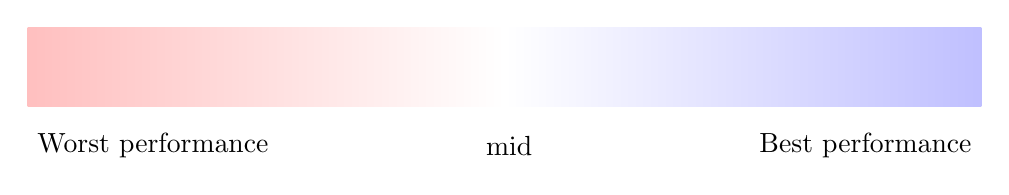
\begin{tikzpicture}%[remember picture,overlay]
\node[right] (start) at (0,-0.5) {Worst performance};
\node[left] (end) at (\linewidth-\pgflinewidth,-0.5) {Best performance};
\node[] (mid) at ($(start)!0.5!(end)$) {mid};
\path[left color=worstclr!25, right color=bestclr!25,middle color=avgclr!25]
(0,0) rectangle ++(\linewidth-\pgflinewidth,1); 
\end{tikzpicture}
\caption{Throughout this section we use these colours to highlight numbers, to make it easier to compare the numbers. The range is best on both the \textcolor{worstclr!50}{worst performance}, and the \textcolor{bestclr!50}{best performance}. We use a linear scale (even though for perplexity a log scale might be more appropriate).}
\label{fig:colourrange}
\end{figure}

\subsection{Skipgrams and perplexity reductions}
The first comparison is between \textsf{ngram} and \textsf{uni}, since these backoff strategies embody the difference between only $n$-gram features (\textsf{ngram}), and both $n$-gram and skipgram features (\textsf{uni}). We report the perplexities in \cref{tab:ngramsvsskipgrams}, and the relative difference in perplexity when choosing skipgrams\footnote{Read, skipgrams and $n$-grams. In our experiments we never use only skipgrams. We use this convention in the remainder of this thesis, except in cases where there might be some ambiguity otherwise.} over $n$-grams.

\npdecimalsign{.}
\nprounddigits{0}
\begin{table}[]
	\centering
	\caption{My caption}
	\label{tab:ngramsvsskipgrams}
	\begin{tabular}{lllllllllllllll}
		training & \multicolumn{4}{c}{1bw}            &  & \multicolumn{4}{c}{emea} &  & \multicolumn{4}{c}{jrc}             \\
		test     & 1bw  & emea  & jrc  & wp    
		      &  & 1bw  & emea  & jrc  & wp 
		      &  & 1bw  & emea  & jrc  & wp      \\
		\textsf{ngram}   & \btc{25}\numprint{129.47} &  \numprint{1123.89} 
					&  \numprint{941.4}  &  \numprint{456.27} &  
		        & \numprint{1761.34} & \numprint{5.63033} 
		            & \numprint{898} & \numprint{1123.58} &  
		        &  \numprint{1520.1}  &  \numprint{1278.94} 
			         &  \btc{25}\numprint{12.85} &  \numprint{1249.28} \\
		\textsf{fulluni}  & \numprint{124.69} & \numprint{728.27}  
				 	& \numprint{728.98} & \numprint{392.04} 
				 &  & \numprint{1393.81} & \numprint{5.6754} 
				 	& \numprint{773.116} & \numprint{907.558} &  
				 & \numprint{1303.66} & \numprint{1069.64} 
				 	& \btc{25}\numprint{13.32} & \numprint{1067.99} \\
		$\Delta$\% & \numprint{3.1} & \numprint{35.23} & \numprint{22.53}   &  \numprint{14.04}
				& & \numprint{20.840} & \numprint{-0.800} 
					& \numprint{13.91982} & \numprint{19.217} &
				& \numprint{14.21} & \numprint{16.34} & \numprint{-3.65} & \numprint{14.49} \\
	\end{tabular}
\end{table}

\subsection{Interpolation between $n$-grams and skipgrams}
The previous results show that if we add skipgrams, we can reduce the perplexity. Since \textsf{uni} is a very naive prior weight, in this section we investigate the effect of adding weights as interpolation factors.

If we would have enough training material, skipgrams might not be necessary, as all information is then captured by the $n$-grams. This hypothesis suggests that $n$-grams carry more information, and in cases where $n$-grams do not cover the encountered patterns, skipgrams are an additional help.

An initial guess for $n$-gram preference was a ratio of 2:1, in favour of $n$-grams. The results for \textsf{fullnpref}\footnote{Unless otherwise noted for \textsf{fullnpref}, the preference ratio is 2.0.} are shown in \cref{tab:fullunivsfullnpref2}, show around 5\% reductions in perplexity compared to \textsf{fulluni}. Although in itself the reductions are not that impressive, they are combined with the reductions in \cref{tab:ngramsvsskipgrams}.

\begin{table}[]
	\centering
	\caption{My caption}
	\label{tab:fullunivsfullnpref2}
	\begin{tabular}{lllllllllllllll}
		training & \multicolumn{4}{c}{\obw}            &  & \multicolumn{4}{c}{\emea} &  & \multicolumn{4}{c}{\jrc}             \\
		test     & \obw  & \emea  & \jrc  & \wp    
		&  & \obw  & \emea  & \jrc  & \wp 
		&  & \obw  & \emea  & \jrc  & \wp      \\
		\textsf{fulluni}   & \numprint{124.69} &  \numprint{728.27} 
		&  \numprint{728.98}  &  \numprint{392.04} &  
		& \numprint{1393.81} & \numprint{5.6754} 
			& \numprint{773.116} & \numprint{907.558} &  
		&  \numprint{1303.66}  &  \numprint{1069.64} 
		&  \numprint{13.32} &  \numprint{1067.99} \\
		\textsf{fullnpref}  & \numprint{118.28} & \numprint{699.91}  
		& \numprint{694.32} & \numprint{372.06} 
		&  & \numprint{1305.9} &  \numprint{5.59}     
		  & \numprint{704.94} & \numprint{852.52}   &  
		& \numprint{1215.52} & \numprint{1000.72} 
		& \numprint{12.84} & \numprint{1000} \\
		$\Delta$\% & \numprint{5.6} & \numprint{3.85} & \numprint{4.80}   &  \numprint{5.10}
		& &\numprint{6.312769}&\numprint{1.5047}
			&\numprint{8.796895}&\numprint{6.0572687}&
		& \numprint{6.75} & \numprint{6.45} & \numprint{3.6} & \numprint{6.37} \\
	\end{tabular}
\end{table}

Even with these positive results, it is hard to not verify whether 2.0 is indeed the optimal value for \textsf{fullnpref}. In \cref{tab:nprefgrid} we show the results of a search for the lowest perplexity, in 25 steps in the logarithmic space from 0.05 through 20.

\begin{table*}\resizebox{\columnwidth}{!}{%
		\begin{tabular}{llllllllllllllllllllllllll}
			\textsf{fullnpref} & 0.05 & 0.06 & 0.08 & 0.11 & 0.14 & 0.17 & 0.22 & 0.29 & 0.37 & 0.47 & 0.61 & 0.78 & 1 & 1.28 & 1.65 & 2.11 & 2.71 & 3.48 & 4.47 & 5.73 & 7.36 & 9.44 & 12.12 & 15.55 & 19.95 \\
			\obw & \wtc{19.4295700804}\numprint{170.844} & \wtc{17.642782244}\numprint{168.288} & \wtc{14.6752883607}\numprint{164.043} & \wtc{11.2023767913}\numprint{159.075} & \wtc{8.46696959105}\numprint{155.162} & \wtc{6.21740650122}\numprint{151.944} & \wtc{3.19328905977}\numprint{147.618} & \btc{0.045438657812}\numprint{142.985} & \btc{2.85424676686}\numprint{138.967} & \btc{5.52114645229}\numprint{135.152} & \btc{8.27123383432}\numprint{131.218} & \btc{10.6641034603}\numprint{127.795} & \btc{12.8381684726}\numprint{124.685} & \btc{14.7165326809}\numprint{121.998} & \btc{16.3257602237}\numprint{119.696} & \btc{17.5567983223}\numprint{117.935} & \btc{18.4781544914}\numprint{116.617} & \btc{19.0772457183}\numprint{115.76} & \btc{19.38273331}\numprint{115.323} & \btc{19.4295700804}\numprint{115.256} & \btc{19.2590003495}\numprint{115.5} & \btc{18.9171618315}\numprint{115.989} & \btc{18.4445997903}\numprint{116.665} & \btc{17.8818594897}\numprint{117.47} & \btc{17.2645927997}\numprint{118.353} \\
			\emea & \wtc{19.7839277582}\numprint{1041.55} & \wtc{17.6333258196}\numprint{1022.85} & \wtc{14.0817274739}\numprint{991.968} & \wtc{9.95820701901}\numprint{956.113} & \wtc{6.74000947645}\numprint{928.13} & \wtc{4.1170801496}\numprint{905.323} & \wtc{0.633565030982}\numprint{875.033} & \btc{3.03234873333}\numprint{843.157} & \btc{6.13979602633}\numprint{816.137} & \btc{9.01194216606}\numprint{791.163} & \btc{11.8682175535}\numprint{766.327} & \btc{14.2343397077}\numprint{745.753} & \btc{16.2455550393}\numprint{728.265} & \btc{17.8203246834}\numprint{714.572} & \btc{18.9673890542}\numprint{704.598} & \btc{19.6067043578}\numprint{699.039} & \btc{19.7839277582}\numprint{697.498} & \btc{19.5042345007}\numprint{699.93} & \btc{18.802701248}\numprint{706.03} & \btc{17.737405753}\numprint{715.293} & \btc{16.3469898473}\numprint{727.383} & \btc{14.7095422323}\numprint{741.621} & \btc{12.8258679461}\numprint{758.0} & \btc{10.8975715449}\numprint{774.767} & \btc{8.84000901643}\numprint{792.658} \\
			\jrc & \wtc{20.9393339638}\numprint{1053.15} & \wtc{18.8263550482}\numprint{1034.75} & \wtc{15.30204402}\numprint{1004.06} & \wtc{11.1624427185}\numprint{968.012} & \wtc{7.90156503985}\numprint{939.616} & \wtc{5.22577581638}\numprint{916.315} & \wtc{1.647606793}\numprint{885.156} & \btc{2.14955412126}\numprint{852.09} & \btc{5.39688117422}\numprint{823.812} & \btc{8.42774272415}\numprint{797.419} & \btc{11.4793895558}\numprint{770.845} & \btc{14.0498743409}\numprint{748.461} & \btc{16.2861869171}\numprint{728.987} & \btc{18.1019707548}\numprint{713.175} & \btc{19.5143363897}\numprint{700.876} & \btc{20.4275107558}\numprint{692.924} & \btc{20.9017826537}\numprint{688.794} & \btc{20.9393339638}\numprint{688.467} & \btc{20.5781753394}\numprint{691.612} & \btc{19.8758395215}\numprint{697.728} & \btc{18.8791795211}\numprint{706.407} & \btc{17.6627237791}\numprint{717.0} & \btc{16.2760813658}\numprint{729.075} & \btc{14.7856273796}\numprint{742.054} & \btc{13.2386741746}\numprint{755.525} \\
			\wp & \wtc{20.7199743005}\numprint{558.048} & \wtc{18.7042539314}\numprint{548.73} & \wtc{15.3451526338}\numprint{533.202} & \wtc{11.4047849022}\numprint{514.987} & \wtc{8.2998659864}\numprint{500.634} & \wtc{5.74982180193}\numprint{488.846} & \wtc{2.33296161413}\numprint{473.051} & \btc{1.30671376792}\numprint{456.226} & \btc{4.43607745748}\numprint{441.76} & \btc{7.37767067265}\numprint{428.162} & \btc{10.3692350625}\numprint{414.333} & \btc{12.9246873827}\numprint{402.52} & \btc{15.1911289267}\numprint{392.043} & \btc{17.0848417525}\numprint{383.289} & \btc{18.6278910542}\numprint{376.156} & \btc{19.7157916483}\numprint{371.127} & \btc{20.4145227915}\numprint{367.897} & \btc{20.7199743005}\numprint{366.485} & \btc{20.666541919}\numprint{366.732} & \btc{20.3035478452}\numprint{368.41} & \btc{19.677502047}\numprint{371.304} & \btc{18.8515715502}\numprint{375.122} & \btc{17.8729152989}\numprint{379.646} & \btc{16.7984268815}\numprint{384.613} & \btc{15.6705060825}\numprint{389.827} \\
			
		\end{tabular}
	}
\caption{The perplexity values for different \textsf{fullnpref} preference rates with the \obw model. The 25 steps were sampled in a log space from $[10^{-1.3},10^{1.3}]$. The results show that indeed \textsf{fullnpref-2.0} was a good first guess, with optimal values somewhere between 2.71 and 4.47, depending on the test set.}
\label{tab:nprefgrid}
\end{table*}

These results to some extent weaken the position of skipgrams, as $n$-grams are given a preference of at least 2 times, up to 4. But nonetheless, the skipgrams contribute to a lower perplexity,\footnote{See \cref{tab:ngramsvsskipgrams,tab:fullunivsfullnpref2}.} where this could not be achieved with solely using $n$-grams.

\subsection{Individual interpolation values per backoff step}
In the previous chapter we graphically introduced the backoff steps in \cref{fig:bof}. If we consider the directed edges in the tree going from one node to a smaller node\footnote{Where we measure the size of a node by the length of a pattern minus the number of skips.}, then for \textsf{uni} the edges are weighted 1, and for \textsf{npref} the edges $w_{d}$, $w_{cd}$, $w_{bcd}$, and $w_{abcd}$ have weight 1, with the others being 2.

In the following example we convert the graph into a tree for a 4-gram model, and we add the names of the backoff weights, corresponding to the terms introduced for \textsf{value} earlier this chapter.

\begin{figure*}
    \begin{tikzpicture}[every node/.style={node distance=10pt, rectangle, minimum size=1cm}]
    
    \node[] (d1) {d};
    \node[below=of d1] (d2) {d};
    \node[below=of d2] (d3) {d};
    \node[below=of d3] (d4) {d};
    \node[below=of d4] (d5) {d};
    \node[below=of d5] (d6) {d};
    
    \node[left=0cm and 2.5cm of d1] (axxd1) {axxd};
    \node[left=0cm and 2.5cm of d3] (axxd2) {axxd};
    \node[left=0cm and 2.5cm of d2] (cd1) {cd};
    \node[left=0cm and 2.5cm of d5] (cd2) {cd};
    \node[left=0cm and 2.5cm of d4] (bxd1) {bxd};
    \node[left=0cm and 2.5cm of d6] (bxd2) {bxd};
    
    \node[left=0cm and 2.5cm of $(axxd1)!0.5!(cd1)$] (axcd) {axcd};
    \node[left=0cm and 2.5cm of $(axxd2)!0.5!(bxd1)$] (abxd) {abxd};
    \node[left=0cm and 2.5cm of $(cd2)!0.5!(bxd2)$] (bcd) {bcd};
    
    \node[left=0cm and 2.5cm of abxd] (abcd) {abcd};
    
    \draw (abcd) -- node[above] {$w_{axcd}$} ++ (axcd);
    \draw (abcd) -- node[above] {$w_{abxd}$} ++ (abxd);
    \draw (abcd) -- node[below] {$w_{bcd}$} ++ (bcd);
    
    \draw (axcd) -- node[above] {$w_{axxd}$} ++ (axxd1);
    \draw (axcd) -- node[below] {$w_{cd}$} ++ (cd1);
    \draw (abxd) -- node[above] {$w_{axxd}$} ++ (axxd2);
    \draw (abxd) -- node[below] {$w_{bxd}$} ++ (bxd1);
    \draw (bcd) -- node[above] {$w_{cd}$} ++ (cd2);
    \draw (bcd) -- node[below] {$w_{bxd}$} ++ (bxd2);
    
    \draw (axxd1) -- node[below] {$w_d$} ++ (d1);
    \draw (cd1) -- node[below] {$w_d$} ++ (d2);
    \draw (axxd2) -- node[below] {$w_d$} ++ (d3);
    \draw (bxd1) -- node[below] {$w_d$} ++ (d4);
    \draw (cd2) -- node[below] {$w_d$} ++ (d5);
    \draw (bxd2) -- node[below] {$w_d$} ++ (d6);
   	\end{tikzpicture}
    \caption{}
    \label{fig:value}
    \end{figure*}


\subsection{A qualitative analysis into the contribution of skipgrams}

%\section{Experiments}
%We train 4-gram language model on the two training corpora, the Google 1 billion word benchmark and the Mediargus corpus.\footnote{See~\cref{sec:data} for a description of the corpora.} We do not perform any preprocessing on the data except tokenisation. 
%   %The models are trained with a HPYLM. We do not use sentence beginning and end markers. The results for the {\sf ngram} backoff strategy are obtained by training without skipgrams; for {\sf limited} and {\sf full} we added skipgram features during training.
%
%When setting up the experimental framework, we had to decide on the basis. Earlier work on hierarchical Pitman-Yor language models by Huang and Renals had accompanying software releases. An SRILM extension with HPYPLM was proposed in \autocite{huang2007hierarchical}, and a frequentist approximation extension of the HPYPLM was described in \autocite{huang2010power}. However, at the time I started this thesis, they were no longer accessible. With further inquiries we learned that also none of the source code has survived during the period. 
%
%We found an alternative in cpyp,\footnote{\url{https://github.com/redpony/cpyp}} which is an existing library for non-parametric Bayesian modelling with PY priors with histogram-based sampling \cite{blunsom2009note}. This library has an example application to showcase its performance with $n$-gram based language modelling. Limitations of the library, such as not natively supporting skipgrams, and the lack of other functionality such as thresholding and discarding of certain patterns, led us to extend the library with Colibri Core,\footnote{\url{http://proycon.github.io/colibri-core/}} a pattern modelling library. Colibri Core resolves the limitations, and together the libraries are a complete language model that handles skipgrams: cococpyp.\footnote{\url{https://github.com/naiaden/cococpyp}} This software in turn has been rewritten to allow also for reranking nbest lists, and being more in control of the underlying language model. We gave it the name SLM, for skipgram language model.\footnote{\url{https://github.com/naiaden/SLM}} Throughout the rest of the thesis the reported results were obtained with SLM.
%
%  Each model is run for 50 iterations (without an explicit burn-in phase), with the initial values for hyperparameters $\theta=1.0$ and $\gamma=0.8$. The hyperparameters are resampled every 30 iterations with slice sampling \cite{walker2007sampling}.
%  
%  \textbf{Plot van dalende ppl over iteraties, effect resampling?}
%  
%  We test each model on different test sets, and we collect their intrinsic performance by means of perplexity. We compute the perplexity on all 4-grams, rather than computing the perplexity for sentences. 
%  Words in the test set that were unseen in the training data are ignored in computing the perplexity on test data.\footnote{This is common for perplexity. } 

\subsection{PPL}
\subsection{Learning curves}

\section{Results}

\section{Discussion}
%%\chapter{Domain-adaptation with a double hierarchical Pitman-Yor skipgram language model}

%%\part{Extrinsic evaluation}
%%\chapter{Chapter 4\newline The influence of skipgrams on automatic speech recognition}\label{ch:speech}
%%\chapter{Relating brain activity data to perplexities from skipgram models}
%%\chapter{Using skipgram language models in automatic speech recognition for under-resourced languages}

%\chapter{Conclusion}



%%%
%% The back matter contains appendices, bibliographies, indices, glossaries, etc.

\backmatter

\appendix
\chapter{Derivation and proof for the hierarchical Pitman-Yor process language model with added interpolation factors and backoff strategies}\label{apx:proofinterpolform}

In the original paper by Teh,\autocite{teh2006hierarchical} the functions\footnote{Ibidem, Equations 10 and 11.} that return the word probability are defined as:

\begin{equation}
\begin{split}
p(w | 0, \mathcal{S}, \Theta) =& 1/V \\
p(w | \mathbf{u}, \mathcal{S}, \Theta) =& \frac{c_{\mathbf{u}w\cdot} - d_{|\mathbf{u}|}t_{\mathbf{u}w\cdot}}{\theta_{|\mathbf{u}|}+c_{\mathbf{u}\cdot\cdot}} + \frac{\theta_{|\mathbf{u}|} + d_{|\mathbf{u}|}t_{\mathbf{u}\cdot\cdot}}{\theta_{|\mathbf{u}|}+c_{\mathbf{u}\cdot\cdot}} p(w | \pi(\mathbf{u}), \mathcal{S}, \Theta)
\end{split}
\end{equation}

With each extension to these formulae, we have to proof that the result is a proper probability distribution again.\footnote{Non-normalised language models are also use, i.e.\ Stupid Backoff \autocite{brants2007large}.}

Since these formulae will serve as the basis for our \textsl{limited} backoff strategy, we show its correctness. A step we also have to show for our derivation.

We show its correctness by showing that the probability distribution sums up to one (and that it is not negative, and the elements are not bigger than 1).

Assume there is a dictionary $W$ with $V$ words. Then we can sum over all customers in each restaurant, for all dishes with $\sum_{w\in W} c_{\mathbf{u}w} = c_{\mathbf{u}\cdot\cdot}$, and similarly for the tables: $\sum_{w\in W} t_{\mathbf{u}w\cdot} = t_{\mathbf{u}\cdot\cdot}$. 
\begin{equation}
\begin{split}
	\sum_{w\in W} p(w | \mathbf{u}, \mathcal{S}, \Theta) = 1 \\
    \sum_{w\in W}\frac{c_{\mathbf{u}w\cdot} - d_{|\mathbf{u}|}t_{\mathbf{u}w\cdot}}{\theta_{|\mathbf{u}|}+c_{\mathbf{u}\cdot\cdot}} + \frac{\theta_{|\mathbf{u}|} + d_{|\mathbf{u}|}t_{\mathbf{u}\cdot\cdot}}{\theta_{|\mathbf{u}|}+c_{\mathbf{u}\cdot\cdot}} p(w | \pi(\mathbf{u}), \mathcal{S}, \Theta) = 1 \\
    \sum_{w\in W}\frac{c_{\mathbf{u}w\cdot} - d_{|\mathbf{u}|}t_{\mathbf{u}w\cdot}}{\theta_{|\mathbf{u}|}+c_{\mathbf{u}\cdot\cdot}} + \sum_{w\in W} \frac{\theta_{|\mathbf{u}|} + d_{|\mathbf{u}|}t_{\mathbf{u}\cdot\cdot}}{\theta_{|\mathbf{u}|}+c_{\mathbf{u}\cdot\cdot}} p(w | \pi(\mathbf{u}), \mathcal{S}, \Theta) =1 \\
    \sum_{w\in W} \frac{c_{\mathbf{u}w\cdot}}{\theta_{|\mathbf{u}|}+c_{\mathbf{u}\cdot\cdot}} - \sum_{w\in W} \frac{d_{|\mathbf{u}|}t_{\mathbf{u}w\cdot}}{\theta_{|\mathbf{u}|}+c_{\mathbf{u}\cdot\cdot}} + \sum_{w\in W} \frac{\theta_{|\mathbf{u}|}p(w | \pi(\mathbf{u}), \mathcal{S}, \Theta)}{\theta_{|\mathbf{u}|}+c_{\mathbf{u}\cdot\cdot}} + \sum_{w\in W} \frac{d_{|\mathbf{u}|}t_{\mathbf{u}\cdot\cdot} p(w | \pi(\mathbf{u}), \mathcal{S}, \Theta)}{\theta_{|\mathbf{u}|}+c_{\mathbf{u}\cdot\cdot}} = 1 \\
    \frac{c_{\mathbf{u}\cdot\cdot}}{\theta_{|\mathbf{u}|}+c_{\mathbf{u}\cdot\cdot}} - \frac{d_{|\mathbf{u}|}t_{\mathbf{u}\cdot\cdot}}{\theta_{|\mathbf{u}|}+c_{\mathbf{u}\cdot\cdot}} + \theta_{|\mathbf{u}|}\sum_{w\in W} \frac{p(w | \pi(\mathbf{u}), \mathcal{S}, \Theta)}{\theta_{|\mathbf{u}|}+c_{\mathbf{u}\cdot\cdot}} + d_{|\mathbf{u}|}t_{\mathbf{u}\cdot\cdot}\sum_{w\in W} \frac{ p(w | \pi(\mathbf{u}), \mathcal{S}, \Theta)}{\theta_{|\mathbf{u}|}+c_{\mathbf{u}\cdot\cdot}} = 1 \\
    \frac{c_{\mathbf{u}\cdot\cdot}}{\theta_{|\mathbf{u}|}+c_{\mathbf{u}\cdot\cdot}} - \frac{d_{|\mathbf{u}|}t_{\mathbf{u}\cdot\cdot}}{\theta_{|\mathbf{u}|}+c_{\mathbf{u}\cdot\cdot}} +\frac{ \theta_{|\mathbf{u}|}}{\theta_{|\mathbf{u}|}+c_{\mathbf{u}\cdot\cdot}} + \frac{ d_{|\mathbf{u}|}t_{\mathbf{u}\cdot\cdot}}{\theta_{|\mathbf{u}|}+c_{\mathbf{u}\cdot\cdot}} = 1 \\
    \frac{c_{\mathbf{u}\cdot\cdot}- d_{|\mathbf{u}|}t_{\mathbf{u}\cdot\cdot}}{\theta_{|\mathbf{u}|}+c_{\mathbf{u}\cdot\cdot}} = 1
\end{split}
\end{equation}

For the limited backoff method we distinguish between the word probability, and the backoff probability and its weight. If a pattern $\mathbf{u}w$ occurs in the training data, we only use the word probability, and otherwise we use the word probability with its weighted backoff probability.

Assume that we have a context pattern $\mathbf{u}$, and a vocabulary of $V$ words, of which $N$ words $w$ occur in the training data as $\mathbf{u}w$. $B$ of the $V$ words do not occur, hence $V = N + B$\marginnote{Read $B$ as backoff when this pattern occurs, and $N$ as no backoff}. 
If we naively ignore the backoff probability in the $N$ cases, then the probability distribution does not sum up to one anymore.

In the following example we show that our extension is a proper distribution. Let's call the words that we don't backoff for $\mathcal{N}$, and the other words $\mathcal{B}$. In the proof we will skip over the steps that are already in the previous example.

Note that we can compute $\sum_{w\in\mathcal{B}} p(w|\pi(\mathbf{u}), \mathcal{S}, \Theta) = P$, and that this does not sum up to one. So we add a term $Q = 1 - P$.

\begin{equation}
\begin{split}
	\sum_{w\in W} p(w | \mathbf{u}, \mathcal{S}, \Theta) = 1 \\
    \sum_{w\in\mathcal{N}} p(w | \mathbf{u}, \mathcal{S}, \Theta) + \sum_{w\in\mathcal{B}} p(w | \mathbf{u}, \mathcal{S}, \Theta) = 1 \\
    \sum_{w\in\mathcal{N}}\frac{c_{\mathbf{u}w\cdot} - d_{|\mathbf{u}|}t_{\mathbf{u}w\cdot}}{\theta_{|\mathbf{u}|}+c_{\mathbf{u}\cdot\cdot}} + \frac{\theta_{|\mathbf{u}|} + d_{|\mathbf{u}|}t_{\mathbf{u}\cdot\cdot}}{\theta_{|\mathbf{u}|}+c_{\mathbf{u}\cdot\cdot}} q + \sum_{w\in\mathcal{B}}\frac{c_{\mathbf{u}w\cdot} - d_{|\mathbf{u}|}t_{\mathbf{u}w\cdot}}{\theta_{|\mathbf{u}|}+c_{\mathbf{u}\cdot\cdot}} + \frac{\theta_{|\mathbf{u}|} + d_{|\mathbf{u}|}t_{\mathbf{u}\cdot\cdot}}{\theta_{|\mathbf{u}|}+c_{\mathbf{u}\cdot\cdot}} p(w | \pi(\mathbf{u}), \mathcal{S}, \Theta) = 1 \\
	\frac{\sum_{w\in\mathcal{N}}c_{\mathbf{u}w\cdot} + \sum_{w\in\mathcal{B}}c_{\mathbf{u}w\cdot}}{\theta_{|\mathbf{u}|}+c_{\mathbf{u}\cdot\cdot}} - \frac{\sum_{w\in\mathcal{N}}d_{|\mathbf{u}|}t_{\mathbf{u}w\cdot} + \sum_{w\in\mathcal{B}}d_{|\mathbf{u}|}t_{\mathbf{u}w\cdot}}{\theta_{|\mathbf{u}|}+c_{\mathbf{u}\cdot\cdot}} + \sum_{w\in\mathcal{N}}\frac{\theta_{|\mathbf{u}|} + d_{|\mathbf{u}|}t_{\mathbf{u}\cdot\cdot}}{\theta_{|\mathbf{u}|}+c_{\mathbf{u}\cdot\cdot}} q + \sum_{w\in\mathcal{B}}\frac{\theta_{|\mathbf{u}|} + d_{|\mathbf{u}|}t_{\mathbf{u}\cdot\cdot}}{\theta_{|\mathbf{u}|}+c_{\mathbf{u}\cdot\cdot}} p(w | \pi(\mathbf{u}), \mathcal{S}, \Theta)= 1\\
    \frac{c_{\mathbf{u}\cdot\cdot}}{\theta_{|\mathbf{u}|}+c_{\mathbf{u}\cdot\cdot}} - \frac{d_{|\mathbf{u}|}t_{\mathbf{u}\cdot\cdot}}{\theta_{|\mathbf{u}|}+c_{\mathbf{u}\cdot\cdot}} + \sum_{w\in\mathcal{N}}\frac{\theta_{|\mathbf{u}|} + d_{|\mathbf{u}|}t_{\mathbf{u}\cdot\cdot}}{\theta_{|\mathbf{u}|}+c_{\mathbf{u}\cdot\cdot}} q + \sum_{w\in\mathcal{B}}\frac{\theta_{|\mathbf{u}|} + d_{|\mathbf{u}|}t_{\mathbf{u}\cdot\cdot}}{\theta_{|\mathbf{u}|}+c_{\mathbf{u}\cdot\cdot}} p(w | \pi(\mathbf{u}), \mathcal{S}, \Theta)= 1 \\
    \frac{c_{\mathbf{u}\cdot\cdot}}{\theta_{|\mathbf{u}|}+c_{\mathbf{u}\cdot\cdot}} - \frac{d_{|\mathbf{u}|}t_{\mathbf{u}\cdot\cdot}}{\theta_{|\mathbf{u}|}+c_{\mathbf{u}\cdot\cdot}} + \sum_{w\in\mathcal{N}}\frac{d_{|\mathbf{u}|}t_{\mathbf{u}\cdot\cdot}}{\theta_{|\mathbf{u}|}+c_{\mathbf{u}\cdot\cdot}} q + \sum_{w\in\mathcal{N}}\frac{\theta_{|\mathbf{u}|}}{\theta_{|\mathbf{u}|}+c_{\mathbf{u}\cdot\cdot}} q + \sum_{w\in\mathcal{B}}\frac{\theta_{|\mathbf{u}|} + d_{|\mathbf{u}|}t_{\mathbf{u}\cdot\cdot}}{\theta_{|\mathbf{u}|}+c_{\mathbf{u}\cdot\cdot}} p(w | \pi(\mathbf{u}), \mathcal{S}, \Theta)= 1 \\
    \frac{c_{\mathbf{u}\cdot\cdot}}{\theta_{|\mathbf{u}|}+c_{\mathbf{u}\cdot\cdot}} - \frac{d_{|\mathbf{u}|}t_{\mathbf{u}\cdot\cdot}}{\theta_{|\mathbf{u}|}+c_{\mathbf{u}\cdot\cdot}} +  \frac{d_{|\mathbf{u}|}t_{\mathbf{u}\cdot\cdot}Q}{\theta_{|\mathbf{u}|}+c_{\mathbf{u}\cdot\cdot}} + \frac{\theta_{|\mathbf{u}|}Q}{\theta_{|\mathbf{u}|}+c_{\mathbf{u}\cdot\cdot}} + \sum_{w\in\mathcal{B}}\frac{\theta_{|\mathbf{u}|} + d_{|\mathbf{u}|}t_{\mathbf{u}\cdot\cdot}}{\theta_{|\mathbf{u}|}+c_{\mathbf{u}\cdot\cdot}} p(w | \pi(\mathbf{u}), \mathcal{S}, \Theta)= 1 \\
    \frac{c_{\mathbf{u}\cdot\cdot}}{\theta_{|\mathbf{u}|}+c_{\mathbf{u}\cdot\cdot}} - \frac{d_{|\mathbf{u}|}t_{\mathbf{u}\cdot\cdot}}{\theta_{|\mathbf{u}|}+c_{\mathbf{u}\cdot\cdot}} +  \frac{d_{|\mathbf{u}|}t_{\mathbf{u}\cdot\cdot}Q}{\theta_{|\mathbf{u}|}+c_{\mathbf{u}\cdot\cdot}} + \frac{\theta_{|\mathbf{u}|}Q}{\theta_{|\mathbf{u}|}+c_{\mathbf{u}\cdot\cdot}} + \theta_{|\mathbf{u}|}\sum_{w\in\mathcal{B}}\frac{p(w | \pi(\mathbf{u}), \mathcal{S}, \Theta)}{\theta_{|\mathbf{u}|}+c_{\mathbf{u}\cdot\cdot}}  + d_{|\mathbf{u}|}t_{\mathbf{u}\cdot\cdot}\sum_{w\in\mathcal{B}}\frac{ p(w | \pi(\mathbf{u}), \mathcal{S}, \Theta)}{\theta_{|\mathbf{u}|}+c_{\mathbf{u}\cdot\cdot}}= 1 \\ 
    \frac{c_{\mathbf{u}\cdot\cdot}}{\theta_{|\mathbf{u}|}+c_{\mathbf{u}\cdot\cdot}} - \frac{d_{|\mathbf{u}|}t_{\mathbf{u}\cdot\cdot}}{\theta_{|\mathbf{u}|}+c_{\mathbf{u}\cdot\cdot}} +  \frac{d_{|\mathbf{u}|}t_{\mathbf{u}\cdot\cdot}Q}{\theta_{|\mathbf{u}|}+c_{\mathbf{u}\cdot\cdot}} + \frac{\theta_{|\mathbf{u}|}Q}{\theta_{|\mathbf{u}|}+c_{\mathbf{u}\cdot\cdot}} + \frac{\theta_{|\mathbf{u}|}P}{\theta_{|\mathbf{u}|}+c_{\mathbf{u}\cdot\cdot}}  + \frac{ d_{|\mathbf{u}|}t_{\mathbf{u}\cdot\cdot}P}{\theta_{|\mathbf{u}|}+c_{\mathbf{u}\cdot\cdot}}= 1 \\
    \frac{c_{\mathbf{u}\cdot\cdot}}{\theta_{|\mathbf{u}|}+c_{\mathbf{u}\cdot\cdot}} + \frac{(-1+P+Q)d_{|\mathbf{u}|}t_{\mathbf{u}\cdot\cdot}}{\theta_{|\mathbf{u}|}+c_{\mathbf{u}\cdot\cdot}} +  \frac{(P+Q)\theta_{|\mathbf{u}|}}{\theta_{|\mathbf{u}|}+c_{\mathbf{u}\cdot\cdot}} = \frac{\theta_{|\mathbf{u}|} + c_{\mathbf{u}\cdot\cdot}}{\theta_{|\mathbf{u}|}+c_{\mathbf{u}\cdot\cdot}}  = 1
\end{split}\label{app:der}
\end{equation}



%\bibliography{superpaper}
%\bibliographystyle{plainnat}

\printbibliography

%\chapter{Samenvating}

\cleardoublepage
\chapter{Summary}
%\input{cv}
%\input{siks}


%\printindex

%\makeatletter
%\protected@write\@auxout{}{%
%  \protect\providecommand\protect\@begindocumenthook{}% Make sure \@begindocumenthook is defined
%  \protect\g@addto@macro\protect\@begindocumenthook{\protect\pgfkeys{%
%  		 /obw/min/obw=\pgfkeysvalueof{/obw/min/obw},%
%         /obw/max/obw=\pgfkeysvalueof{/obw/max/obw},%
%         /obw/min/emea=\pgfkeysvalueof{/obw/min/emea},%
%         /obw/max/emea=\pgfkeysvalueof{/obw/max/emea},%
%         /obw/min/jrc=\pgfkeysvalueof{/obw/min/jrc},%
%         /obw/max/jrc=\pgfkeysvalueof{/obw/max/jrc},%
%         /obw/min/wp=\pgfkeysvalueof{/obw/min/wp},%
%         /obw/max/wp=\pgfkeysvalueof{/obw/max/wp},%
%         /emea/min/obw=\pgfkeysvalueof{/emea/min/obw},%
%         /emea/max/obw=\pgfkeysvalueof{/emea/max/obw},%
%         /emea/min/emea=\pgfkeysvalueof{/emea/min/emea},%
%         /emea/max/emea=\pgfkeysvalueof{/emea/max/emea},%
%         /emea/min/jrc=\pgfkeysvalueof{/emea/min/jrc},%
%         /emea/max/jrc=\pgfkeysvalueof{/emea/max/jrc},%
%         /emea/min/wp=\pgfkeysvalueof{/emea/min/wp},%
%         /emea/max/wp=\pgfkeysvalueof{/emea/max/wp},%
%  		 /jrc/min/obw=\pgfkeysvalueof{/jrc/min/obw},%
%         /jrc/max/obw=\pgfkeysvalueof{/jrc/max/obw},%
%         /jrc/min/emea=\pgfkeysvalueof{/jrc/min/emea},%
%         /jrc/max/emea=\pgfkeysvalueof{/jrc/max/emea},%
%         /jrc/min/jrc=\pgfkeysvalueof{/jrc/min/jrc},%
%         /jrc/max/jrc=\pgfkeysvalueof{/jrc/max/jrc},%
%         /jrc/min/wp=\pgfkeysvalueof{/jrc/min/wp},%
%         /jrc/max/wp=\pgfkeysvalueof{/jrc/max/wp},%
%         }}
%}
%\makeatother

\end{document}
